% ============================================================
%  Shared preamble - matches the Mode-1 / Mode-2 / Mode-3 report house style
% ============================================================
\documentclass[11pt,a4paper]{article}

\usepackage[utf8]{inputenc}
\usepackage[expansion=false]{microtype}
\usepackage[a4paper,left=28mm,right=28mm,top=28mm,bottom=25mm]{geometry}

\usepackage{amsmath,amssymb}
\usepackage{pifont}
\newcommand{\checkmarkx}{\ding{51}}
\usepackage{booktabs}
\usepackage{array}
\usepackage{enumitem}
\usepackage{xcolor}
\usepackage{caption}
\usepackage{fancyhdr}
\usepackage{titlesec}
\usepackage{tikz}
\usetikzlibrary{positioning,arrows.meta,calc,fit,backgrounds,shapes.geometric}
\usepackage[most]{tcolorbox}
\usepackage[section]{placeins}
\usepackage[hidelinks]{hyperref}

% ---------- colours ----------
\definecolor{navy}{RGB}{26,60,102}
\definecolor{accent}{RGB}{40,92,148}
\definecolor{softblue}{RGB}{232,240,248}
\definecolor{rulegrey}{RGB}{120,130,140}
\definecolor{orangeacc}{RGB}{196,106,48}
\definecolor{boxblue}{RGB}{219,232,244}
\definecolor{tealbox}{RGB}{214,236,238}
\definecolor{greybox}{RGB}{238,240,242}
\definecolor{greenbox}{RGB}{214,238,214}
\definecolor{goldbox}{RGB}{250,236,200}

\hypersetup{
  colorlinks=true, linkcolor=accent, urlcolor=accent, citecolor=accent,
  pdftitle={Bluetooth Channel Sounding Mode-0 Frequency and Timing Calibration},
  pdfsubject={Formal technical report},
}

\titleformat{\section}{\normalfont\Large\bfseries\color{navy}}{\thesection}{0.8em}{}
\titleformat{\subsection}{\normalfont\large\bfseries\color{navy}}{\thesubsection}{0.7em}{}
\titleformat{\subsubsection}{\normalfont\normalsize\bfseries\color{navy}}{\thesubsubsection}{0.6em}{}
\titlespacing*{\section}{0pt}{1.9\baselineskip}{0.8\baselineskip}
\titlespacing*{\subsection}{0pt}{1.2\baselineskip}{0.5\baselineskip}

\captionsetup{font=small,labelfont={bf,color=accent},labelsep=colon,width=0.92\textwidth}
\captionsetup[table]{position=above,skip=4pt}
\captionsetup[figure]{position=below,skip=8pt}

\pagestyle{fancy}
\fancyhf{}
\renewcommand{\headrulewidth}{0.6pt}
\fancyhead[L]{\small Bluetooth CS Mode-0 Frequency and Timing Calibration}
\fancyhead[R]{\small Formal technical report - Revision 1.0}
\fancyfoot[C]{\small\thepage}

\newtcolorbox{callout}[1][]{
  colback=softblue, colframe=accent, boxrule=0.5pt,
  left=6pt,right=6pt,top=5pt,bottom=5pt, arc=1pt, fontupper=\small, #1}
\newtcolorbox{caution}[1][]{
  colback=goldbox, colframe=orangeacc, boxrule=0.5pt,
  left=6pt,right=6pt,top=5pt,bottom=5pt, arc=1pt, fontupper=\small, #1}

\newcolumntype{L}[1]{>{\raggedright\arraybackslash}p{#1}}
\renewcommand{\arraystretch}{1.18}

\newcommand{\us}{\,\ensuremath{\upmu}s}
\newcommand{\FFO}{\mathrm{FFO}}
\newcommand{\FAE}{\mathrm{FAE}}
\newcommand{\PCT}{\mathrm{PCT}}
\newcommand{\Tsy}{T_{SY}}
\newcommand{\Tgd}{T_{GD}}
\newcommand{\Tfm}{T_{FM}}
\newcommand{\Trd}{T_{RD}}
\newcommand{\Tipone}{T_{IP1}}
\newcommand{\code}[1]{\texttt{\small #1}}
\providecommand{\upmu}{\mu}
\newcommand{\core}[1]{\textcolor{rulegrey}{\small[Core 6.3, #1]}}

\tikzset{
  blk/.style   ={draw=navy!70, fill=softblue, rounded corners=1pt, align=center,
                 font=\scriptsize, inner sep=3.5pt, minimum height=8mm},
  pblk/.style  ={draw=navy!70, fill=white, rounded corners=1pt, align=center,
                 font=\scriptsize, inner sep=3.5pt, minimum height=8mm},
  ar/.style    ={-{Latex[length=2mm]}, draw=navy!80, thick},
  dar/.style   ={-{Latex[length=2mm]}, draw=orangeacc, dashed, thin},
  slot/.style  ={draw=navy!55, font=\scriptsize, align=center, minimum height=7mm},
}

% ============================================================
\begin{document}

\thispagestyle{empty}
\vspace*{18mm}
{\color{accent}\small\bfseries FORMAL TECHNICAL REPORT \hfill REVISION 1.0}

\vspace{26mm}
{\raggedright\color{navy}\Huge\bfseries Bluetooth Channel Sounding\par}
\vspace{5mm}
{\raggedright\color{navy}\huge\bfseries Mode-0 Frequency and\\[2mm] Timing Calibration\par}

\vspace{7mm}
\noindent{\raggedright\color{rulegrey}\large What is actually observable when two free-running
oscillators measure each other, why actuation error must be exchanged, single-tone estimation over
80\,\ensuremath{\upmu}s, and what the ranging modes really need from the result\par}

\vspace{12mm}
\noindent\rule{\textwidth}{1pt}

\vspace{4mm}
\noindent
This report is an independent treatment of Channel Sounding Mode-0, written from first principles
rather than derived from earlier drafts. It starts from the only thing a receiver physically
observes --- complex phase rotation against its own reference, timed by its own clock --- and builds
up to the fractional frequency offset that the ranging modes consume. It separates three quantities
that are routinely conflated: the \emph{oscillator} rate offset between the two devices, which is
what scales time and phase downstream; the \emph{actuation} error of each synthesiser, which is a
resolution artefact and is why frequency actuation error has to be communicated between the devices
at all; and the \emph{baseband beat} that is the only thing actually measured. It derives the
single-tone estimator family and its Cram\'er--Rao bound, shows that the thermal floor over the
80\,\ensuremath{\upmu}s tone is about $0.03$\,ppm, and then shows that this floor is not the binding
constraint --- a sign convention, a DC offset, or an untrimmed settling transient each cost more than
the noise does. It closes by quantifying, against the companion Mode-1, Mode-2 and Mode-3 reports,
exactly how much frequency accuracy each downstream mode requires, and therefore when Mode-0 is good
enough and when it is not.

\vfill
\noindent
\begin{tabular}{@{}L{40mm}L{95mm}@{}}
Primary references & Core 6.3, Vol.\ 6, Part A, Sec.\ 3.5; Vol.\ 6, Part H, Sec.\ 4.3.1 \\
Architecture & Core 6.3, Vol.\ 1, Part A, Secs.\ 9.1--9.2 \\
Host interface & Core 6.3, Vol.\ 4, Part E, LE CS Subevent Result event \\
Companion reports & \emph{Mode-1 RTT Estimation}, Rev.\ 1.0;
                    \emph{Mode-2 Phase-Based Ranging}, Rev.\ 1.0;
                    \emph{Mode-3 Combined RTT and PBR}, Rev.\ 1.0 \\
Relationship to prior work & Independent; supersedes nothing. See \S\ref{sec:relationship}. \\
Document type & Scientific and implementation-oriented technical report \\
Revision date & 4 September 2026 \\
\end{tabular}

\newpage
\pagenumbering{roman}

\section*{Abstract}
\addcontentsline{toc}{section}{Abstract}

Mode-0 is the calibration step of Bluetooth Low Energy Channel Sounding
\core{Vol.\ 6, Part H, Sec.\ 4.3.1}. The initiator transmits a \code{CS\_SYNC} packet; after the
interlude period the reflector transmits its own \code{CS\_SYNC}, a guard interval, and then an
unmodulated tone of fixed duration $\Tfm = 80\us$. The initiator measures that tone. From it the
initiator derives two outputs that every later step in the subevent depends on: a frequency scale,
expressed as a fractional frequency offset, and a timing reference that tells it when the reflector's
subsequent transmissions will occur.

The physics is simpler than the terminology suggests, and this report tries to keep the two apart. A
receiver cannot observe radio frequency. It observes a phase that rotates at the difference between
the incoming carrier and its own local oscillator, sampled on its own clock. That difference contains
two physically distinct contributions. The first is the \emph{oscillator rate offset} between the two
devices --- a dimensionless quantity that scales every frequency and every time interval on the link,
and the only thing the ranging modes actually need. The second is the \emph{actuation error} of each
device's synthesiser: a real synthesiser cannot emit exactly the commanded frequency, so it emits the
nearest value it can reach, and the residual is an artefact of frequency resolution with no
connection to clock rate. Because the two contributions are inseparable within a single measurement,
and because each device knows only its own actuation error, the peer's value must be communicated ---
which is precisely why frequency actuation error exists as an exchanged quantity in the
specification, and why it must be removed rather than averaged away.

The report derives the reconstruction from measured baseband beat to received radio frequency, giving
explicit attention to the in-phase/quadrature sign convention, whose inversion silently doubles the
error rather than removing it. It develops the estimator family --- lag-$m$ autocorrelation,
unwrapped-phase least squares, and periodogram refinement --- with their ambiguity limits, and shows
that a lag-64 estimator at a 4\,MHz sample rate wraps at $\pm12.8$\,ppm, which is inside the tolerance
of a legitimate crystal pair. A Cram\'er--Rao analysis gives a thermal floor of $0.032$\,ppm at
20\,dB over the full tone, degrading to $0.043$\,ppm once realistic settling and tail margins are
trimmed. An error budget then shows that this floor is comfortably below what any downstream mode
requires, and that Mode-0 accuracy in practice is decided by systematic effects rather than by noise.

\begin{callout}
\textbf{Status and interpretation.} Normative claims are tied to the cited Bluetooth Core
Specification sections and have been checked against the adopted Core 6.3 text: the fractional
frequency offset relation, the actuation-error semantics and encoding, the step structure and every
timing parameter used here are quoted or derived from it. Estimators, windowing, the
in-phase/quadrature sign convention, quality gates and calibration schemes are not specified and are
representative implementation methods. Three numerical inconsistencies in the surrounding series
material, all now settled against the specification, are recorded in
Section~\ref{sec:discrepancies}. The Bluetooth specification and adopted test specifications remain
authoritative for conformance.
\end{callout}

\newpage
\tableofcontents
\newpage
\pagenumbering{arabic}
\setcounter{page}{1}

% ============================================================
\section{Scope, and the relationship to the earlier Mode-0 report}
\label{sec:relationship}
% ============================================================

\subsection{Relationship to prior work}

A previous Mode-0 report exists in this series at Revision 4.0. This document was written
independently and from first principles, at the author's request, and does not modify, correct or
supersede it. The two are complementary rather than competing: where the earlier report builds a
formal reference-frame apparatus and carries a fully instrumented numerical example through every
intermediate value, this one aims to make the physical content legible first and to state plainly
which parts are specified, which are derived, and which are uncertain.

The two agree on the central reconstruction. Working independently, this report arrives at
Eq.~\eqref{eq:reconstruct}, which is the same relation the earlier report states in its abstract.
That agreement is reported here because it is evidence, not because it is a citation: two derivations
from different starting points reaching the same equation is the strongest check available in the
absence of the specification text itself.

\subsection{What Mode-0 is for}

Mode-0 is not a distance measurement and produces no ranging observable. It exists so that the steps
after it in the same subevent can assume a known frequency and timing relationship between the two
devices \core{Vol.\ 1, Part A, Sec.\ 9.1}. It has two outputs, and reports that name themselves after
only the first tend to under-serve the second.

\begin{enumerate}[leftmargin=1.6em,itemsep=2pt]
  \item \textbf{A frequency scale.} The fractional frequency offset between the two devices'
    references. Mode-1 uses it to rescale the reflector's reported turnaround interval; Mode-2 and
    Mode-3 use it to bound the phase that drifts between their reciprocal measurements; all three use
    it to place the expected carrier so that the peer's transmission lands where the receiver is
    listening.
  \item \textbf{A timing reference.} The reflector's \code{CS\_SYNC} in the Mode-0 step tells the
    initiator when the reflector's transmissions actually occur, against the initiator's own clock.
    Every subsequent step in the subevent is scheduled against that reference, and the receive windows
    of later steps are opened on the strength of it.
\end{enumerate}

\begin{callout}
\textbf{Why the calibration is repeated per subevent.} Neither output is a constant. Reference
oscillators drift with temperature and supply, and the relationship between two of them drifts
faster than either alone. A subevent begins with one to three Mode-0 steps rather than a
procedure-level calibration because the correction must be fresh: what matters is the offset during
\emph{these} ranging steps, not the offset when the procedure started.
\end{callout}

\subsection{Questions this report answers}

\begin{enumerate}[leftmargin=1.6em,itemsep=1pt]
  \item What, exactly, does a receiver physically observe during the Mode-0 tone?
  \item Which part of that observation is the quantity the ranging modes need, and which part is an
        artefact that must be removed?
  \item Why does frequency actuation error have to be exchanged between the devices, rather than
        each device handling its own?
  \item How does phase rotation per sample become a fractional frequency offset, and where does the
        sign come from?
  \item How precisely can the offset be estimated over $80\us$, and what limits it in practice?
  \item How much accuracy does each downstream mode actually require, and does Mode-0 deliver it?
\end{enumerate}
% ============================================================
\section{Normative framework and terminology}
% ============================================================

\begin{table}[h]
\caption{Normative map for Mode-0. Section numbering should be confirmed against the specification
revision in force.}
\label{tab:normmap}
\centering\small
\begin{tabular}{@{}L{42mm}L{51mm}L{51mm}@{}}
\toprule
Source & What it defines & Question answered \\
\midrule
Core 6.3, Vol.\ 1, Part A, Sec.\ 9.1 & CS procedure architecture; the calibration role of the first steps & Why does a subevent begin with Mode-0? \\
Core 6.3, Vol.\ 6, Part H, Sec.\ 4.3.1 & Mode-0 step structure and ordering & What is transmitted, by whom, in what order? \\
Core 6.3, Vol.\ 6, Part H, Sec.\ 4.3 & $\Tsy$, $\Tgd$, $\Tfm$, $\Trd$, $\Tipone$ and permitted values & Which step timings apply? \\
Core 6.3, Vol.\ 6, Part A, Sec.\ 3.5 & Frequency measurement and generation in CS; $f_{RX}[k]$, actuation error, the FFO relation & What is the normative definition of the measured quantity? \\
Core 6.3, Vol.\ 6, Part H, Sec.\ 4.4 & \code{CS\_SYNC} packet construction & What waveform provides the timing reference? \\
Core 6.3, Vol.\ 6, Part B & CS link-layer control procedures, including the exchange of actuation-error data & How does the peer's actuation error reach the receiver? \\
Core 6.3, Vol.\ 4, Part E, LE CS Subevent Result event & Per-step Mode-0 reporting & How is the result exposed to the host? \\
RFPHY.TS / LL.TS, CS Mode-0 clauses & Instrument-level verification & How is the behaviour tested? \\
\bottomrule
\end{tabular}
\end{table}

\begin{table}[h]
\caption{Principal symbols. The decomposition in the middle block is this report's; the
specification's own naming should be preferred where they differ.}
\label{tab:symbols}
\centering\small
\begin{tabular}{@{}L{26mm}L{80mm}L{22mm}@{}}
\toprule
Symbol & Meaning & Units \\
\midrule
$k$ & Mode-0 step index within the subevent & --- \\
$f_{nom}[k]$ & Nominal (commanded) centre frequency of the step's channel & Hz \\
$\varepsilon_I,\ \varepsilon_R$ & Fractional rate error of each device's reference oscillator & --- \\
$\varepsilon$ & Relative oscillator offset $\varepsilon_R-\varepsilon_I$; the quantity sought & --- \\
$\delta_I,\ \delta_R$ & Frequency actuation error of each synthesiser, in its own frame & Hz \\
$f_{LO}^{(I)}[k]$ & Initiator's actual local-oscillator frequency & Hz \\
$f_{TX}^{(R)}[k]$ & Reflector's actual transmitted tone frequency & Hz \\
$\Delta f_{BB}[k]$ & Measured baseband beat frequency & Hz \\
$s_{IQ}$ & In-phase/quadrature sign convention, $\pm1$ & --- \\
$f_{RX}[k]$ & Receiver's estimate of the average received tone frequency & Hz \\
$\FAE$ & Frequency actuation error as communicated between devices & Hz or ppm \\
$\FFO[k]$ & Fractional frequency offset from step $k$ & ppm \\
$\FFO^{*}$ & Subevent fractional frequency offset after combining steps & ppm \\
$z[n]$ & Received complex baseband sample & ADC units \\
$F_s$ & Receiver sample rate (calibrated) & Hz \\
$T_{obs}$ & Accepted observation window inside $\Tfm$ & s \\
$\sigma_f$ & Standard deviation of the frequency estimate & Hz \\
\bottomrule
\end{tabular}
\end{table}

% ============================================================
\section{Numerical inconsistencies in the existing series material}
\label{sec:discrepancies}
% ============================================================

Three parameter conflicts in the surrounding series material were identified while writing this
report and have since been settled directly against Core 6.3. All three are resolved in favour of the
values used here; in every case the timing artwork held with the series is the outlier and should be
corrected.

\begin{caution}
\textbf{(1) $\Tsy$ for a Mode-0 packet: 16\us\ or 26\us?} The Mode-0 timing artwork held with this
series states $\Tsy = 16\us$ in its legend. That value is not reachable from the \code{CS\_SYNC}
packet construction used in the Mode-1 report, which gives, for a packet carrying no sounding or
random sequence, $8+32+4 = 44$ bits on the LE 1M PHY ($44\us$) and $16+32+4 = 52$ bits on the LE 2M
PHY ($26\us$). Sixteen microseconds corresponds to 32 bits at 2\,Mb/s --- the access address alone,
with neither preamble nor trailer.

\emph{Resolved against the specification.} Core 6.3 states that ``CS packets with no Sounding
Sequence or Random Sequence fields take 44\,\ensuremath{\upmu}s to transmit when sent using the LE 1M
PHY and 26\,\ensuremath{\upmu}s to transmit when using the LE 2M and the LE 2M 2BT PHYs''
\core{Vol.\ 6, Part H, Sec.\ 2}, and separately that ``the CS\_SYNCs for mode-0 shall not carry a
sounding sequence or random sequence'' \core{Vol.\ 6, Part H, Sec.\ 4.3.1}. $\Tsy$ for a Mode-0 packet
is therefore $26\us$ on LE 2M and $44\us$ on LE 1M. The artwork's $16\us$ is wrong.
\end{caution}

\begin{caution}
\textbf{(2) $\Tgd$: 3\us\ or 10\us?} The same artwork legend gives a guard delay of $3\us$, while the
earlier Mode-0 report and the campaign report both use $10\us$.

\emph{Resolved against the specification.} Core 6.3 states that ``the guard time (T\_GD) is
10\,\ensuremath{\upmu}s in duration, independent of the LE PHY being used''
\core{Vol.\ 6, Part H, Sec.\ 2.6}. The artwork's $3\us$ is wrong. This also confirms the companion
Mode-3 report's correction to the campaign report's step duration, which is $2\Tgd = 20\us$.
\end{caution}

\begin{caution}
\textbf{(3) The name of the interlude.} The artwork expands $T_{IP,1}$ as ``instantaneous phase
interval''. The interval is an idle period between the two devices' transmissions and carries no
phase measurement; the Mode-1 report calls it the \emph{interlude period}, which matches its
function. Core 6.3 describes $T_{IP1}$ as ``the idle time between the end of the transmission from
the initiator and the start of the transmission from the reflector''
\core{Vol.\ 6, Part H, Sec.\ 4.3.1} --- an idle period, with no phase observable in it. This report
uses ``interlude period''. The distinction is terminological, not numerical, but a reader who takes
the artwork's expansion literally will look for a measurement that does not exist.
\end{caution}

\begin{table}[h]
\caption{Mode-0 step duration under the competing parameter claims, from Eq.~\eqref{eq:stepdur} with
$\Trd=5\us$, $\Tfm=80\us$ and $\Tipone=40\us$. The first row is the specification-confirmed
combination.}
\label{tab:stepcandidates}
\centering\small
\begin{tabular}{@{}L{62mm}rrr@{}}
\toprule
Parameter source & $\Tsy$ & $\Tgd$ & $T_{step,0}$ \\
\midrule
Core 6.3, LE 2M PHY \core{Vol.\ 6, Part H, Secs.\ 2, 2.6} & $26\us$ & $10\us$ & $\mathbf{192\us}$ \\
Timing artwork legend (incorrect) & $16\us$ & $3\us$ & $165\us$ \\
Core 6.3, LE 1M PHY & $44\us$ & $10\us$ & $228\us$ \\
\bottomrule
\end{tabular}
\end{table}

% ============================================================
\section{Step structure and timing}
\label{sec:timing}
% ============================================================

\begin{figure}[h]
\centering
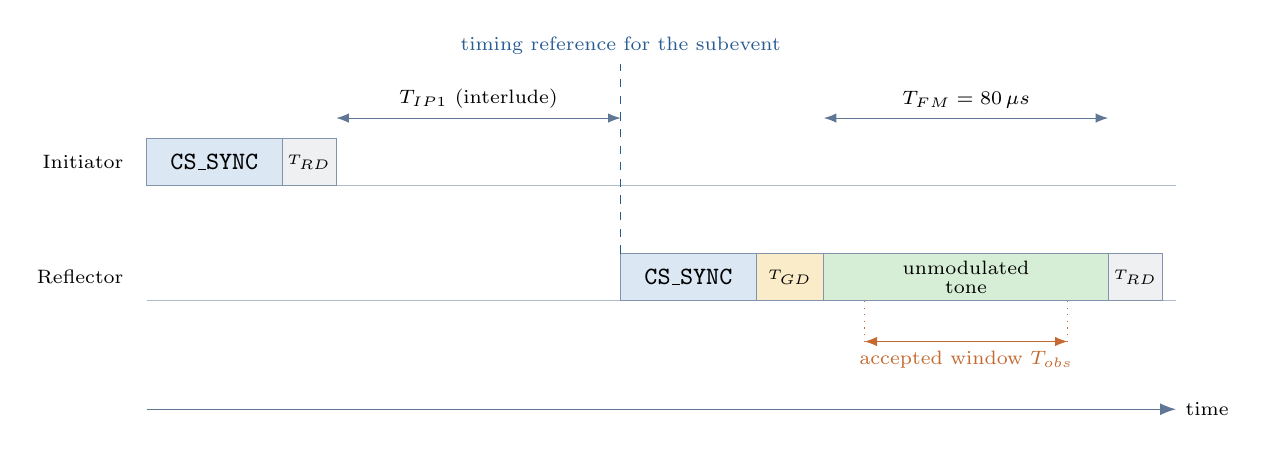
\begin{tikzpicture}[x=0.86mm,y=0.86mm]
\def\yI{17} \def\yR{0}
\draw[-{Latex[length=2mm]},draw=navy!70] (0,\yR-16) -- (152,\yR-16) node[right,font=\scriptsize] {time};
\node[font=\scriptsize,anchor=east] at (-2,\yI+3.5) {Initiator};
\node[font=\scriptsize,anchor=east] at (-2,\yR+3.5) {Reflector};
\draw[draw=navy!35] (0,\yI) -- (152,\yI);
\draw[draw=navy!35] (0,\yR) -- (152,\yR);

% initiator
\draw[slot,fill=boxblue] (0,\yI)  rectangle (20,\yI+7) node[midway] {\code{CS\_SYNC}};
\draw[slot,fill=greybox] (20,\yI) rectangle (28,\yI+7) node[midway,font=\tiny] {$\Trd$};

% reflector
\draw[slot,fill=boxblue] (70,\yR)  rectangle (90,\yR+7) node[midway] {\code{CS\_SYNC}};
\draw[slot,fill=goldbox] (90,\yR)  rectangle (100,\yR+7) node[midway,font=\tiny] {$\Tgd$};
\draw[slot,fill=greenbox](100,\yR) rectangle (142,\yR+7)
      node[midway,align=center] {unmodulated\\[-1pt] tone};
\draw[slot,fill=greybox] (142,\yR) rectangle (150,\yR+7) node[midway,font=\tiny] {$\Trd$};

% interlude bracket
\draw[{Latex[length=1.6mm]}-{Latex[length=1.6mm]},draw=navy!70] (28,\yI+10) -- (70,\yI+10)
   node[midway,above,font=\scriptsize] {$\Tipone$ (interlude)};

% tone duration bracket
\draw[{Latex[length=1.6mm]}-{Latex[length=1.6mm]},draw=navy!70] (100,\yI+10) -- (142,\yI+10)
   node[midway,above,font=\scriptsize] {$\Tfm = 80\us$};

% timing reference
\draw[dashed,draw=accent] (70,\yR+7) -- (70,\yI+18);
\node[font=\scriptsize,color=accent,anchor=south] at (70,\yI+18)
   {timing reference for the subevent};

% measurement window
\draw[{Latex[length=1.6mm]}-{Latex[length=1.6mm]},draw=orangeacc] (106,\yR-6) -- (136,\yR-6)
   node[midway,below,font=\scriptsize,color=orangeacc] {accepted window $T_{obs}$};
\draw[dotted,draw=orangeacc] (106,\yR) -- (106,\yR-6);
\draw[dotted,draw=orangeacc] (136,\yR) -- (136,\yR-6);
\end{tikzpicture}
\caption{Mode-0 step. The initiator's \code{CS\_SYNC} lets the reflector align; the reflector's
\code{CS\_SYNC} gives the initiator its timing reference for the whole subevent, and the $80\us$
unmodulated tone that follows gives it the frequency scale. Only the initiator makes a frequency
measurement. The estimator works on a window strictly inside $\Tfm$, trimmed at both ends
(Section~\ref{sec:window}).}
\label{fig:m0timing}
\end{figure}

The nominal step duration is
\begin{equation}
T_{step,0} \;=\; 2\Tsy \;+\; 2\Trd \;+\; \Tipone \;+\; \Tgd \;+\; \Tfm ,
\label{eq:stepdur}
\end{equation}
which is the expression given in the specification itself
\core{Vol.\ 6, Part H, Sec.\ 4.3.1}, with $\Tfm = 80\us$, $\Tgd = 10\us$ and $\Trd = 5\us$ fixed and
$\Tipone$ configured from the set $\{10,20,30,40,50,60,80,145\}\us$, of which $145\us$ is mandatory
\core{Vol.\ 6, Part H, Table 4.5}. A Mode-0 packet carries no
sounding or random sequence, so $\Tsy$ takes only its shortest value: $26\us$ on the LE 2M PHY and
$44\us$ on LE 1M.

\begin{callout}
\textbf{The step is deliberately asymmetric.} Core 6.3 states that ``the CS initiator performs a
measurement of the frequency offset of the transmitted RF signal from the CS reflector during CS step
mode-0'', and that it ``shall use this information to compensate for the frequency and timing error
contributions in all further transmissions within subsequent CS steps in a CS subevent''
\core{Vol.\ 6, Part H, Sec.\ 4.3.1} --- which also confirms the two outputs of
Section~\ref{sec:relationship}. Unlike every other CS step mode, Mode-0 is not reciprocal. The reflector transmits a tone and the initiator measures it; the reverse measurement is
never made. This is sufficient because the quantity of interest is a \emph{relative} offset, which is
antisymmetric in the two devices: measuring $\varepsilon_R-\varepsilon_I$ once determines
$\varepsilon_I-\varepsilon_R$ as well. It also means the whole of Mode-0's estimation burden falls on
the initiator, and that a reflector-side receiver defect will not show up in Mode-0 at all --- it will
show up later, as a Mode-1 or Mode-2 error with no obvious cause.
\end{callout}

\subsection{Number of steps per subevent}

A subevent begins with one to three Mode-0 steps. More steps buy two different things, and it is
worth separating them: they reduce the variance of the frequency estimate as $1/\sqrt{M}$, and they
give the receiver more than one chance to acquire the timing reference under interference. A design
that is timing-limited and a design that is noise-limited will choose the count for different
reasons.
% ============================================================
\section{What is actually observable}
\label{sec:observable}
% ============================================================

This section builds the measurement from the physics up. It is the core of the report, and everything
later is either estimation theory applied to Eq.~\eqref{eq:beat} or engineering applied to
Eq.~\eqref{eq:ffo}.

\subsection{Two oscillators}

Each device derives everything it does --- its carrier frequencies and its clock ticks alike --- from
one reference oscillator. Let device $X$'s reference run at a fractional rate error $\varepsilon_X$
relative to an ideal reference. This single number scales two things at once, and that coupling
matters later: a device whose reference is fast by $\varepsilon_X$ transmits at frequencies high by
the factor $(1+\varepsilon_X)$ \emph{and} measures time intervals short by the same factor.

Define the relative offset
\begin{equation}
\varepsilon \;\equiv\; \varepsilon_R - \varepsilon_I .
\label{eq:eps}
\end{equation}

\begin{callout}
\textbf{Only $\varepsilon$ is observable, and only $\varepsilon$ is needed.} Neither device can
determine its own $\varepsilon_X$: doing so would require an absolute frequency standard, which
neither has. Nor does either need to. Every downstream use is a comparison between the two devices ---
rescaling the reflector's reported interval onto the initiator's clock, predicting how far the
relative oscillator phase drifts between two measurements, placing a carrier where the peer expects
it --- and every one of those depends on the difference alone. Mode-0 is not a frequency-accuracy
measurement; it is a frequency-\emph{comparison} measurement, and that is why one asymmetric exchange
suffices.
\end{callout}

\subsection{Actuation error: why the commanded frequency is not the emitted one}

A synthesiser cannot emit an arbitrary frequency. It is built from a reference and a divider
structure with finite resolution, so when it is commanded to produce $f_{nom}[k]$ it produces the
nearest value its architecture can reach. Write that residual, expressed in the device's own
reference frame, as the actuation error $\delta_X[k]$. The actual frequencies are then
\begin{align}
f_{TX}^{(R)}[k] &= (1+\varepsilon_R)\bigl(f_{nom}[k] + \delta_R[k]\bigr), \label{eq:ftx}\\
f_{LO}^{(I)}[k] &= (1+\varepsilon_I)\bigl(f_{nom}[k] + \delta_I[k]\bigr). \label{eq:flo}
\end{align}

Two properties of $\delta_X$ drive the whole design. It is \emph{channel-dependent}, because which
frequencies are reachable changes across the band, so it is a table over channels rather than a
constant. And it is \emph{locally knowable}: a device commanded to a frequency knows what its own
synthesiser actually produced, to far better accuracy than it could measure the peer.

\subsection{The beat, and what is in it}

The initiator downconverts the incoming tone against its own local oscillator and observes a complex
baseband signal whose phase rotates at the difference frequency. Subtracting
Eq.~\eqref{eq:flo} from Eq.~\eqref{eq:ftx},
\begin{align}
\Delta f_{true}[k]
 &= (1+\varepsilon_R)(f_{nom}+\delta_R) - (1+\varepsilon_I)(f_{nom}+\delta_I) \nonumber\\
 &= f_{nom}\,\varepsilon \;+\; (\delta_R-\delta_I) \;+\;
    \underbrace{(\varepsilon_R\delta_R - \varepsilon_I\delta_I)}_{\textstyle \text{second order}} .
\label{eq:beat}
\end{align}
The second-order term is the product of a part-per-million quantity and a synthesiser residual of at
most a few hundred hertz; it is below a millihertz and is dropped throughout.

\begin{callout}
\textbf{The one equation that explains the whole of Mode-0's terminology.} Equation~\eqref{eq:beat}
says the measured beat is the sum of two physically unrelated things. The first,
$f_{nom}\varepsilon$, is the oscillator rate offset scaled by the carrier --- the quantity every
ranging mode needs. The second, $\delta_R-\delta_I$, is a difference of synthesiser resolution
artefacts that has nothing to do with clock rate and must not be allowed to masquerade as one. A
single measurement cannot separate them, because they enter identically. Therefore they must be
separated by \emph{knowledge}, not by estimation --- and since the initiator knows only $\delta_I$,
the reflector must tell it $\delta_R$. That exchange is what frequency actuation error is for.
\end{callout}

\subsection{Reconstruction: from baseband beat to received frequency}

What the receiver measures is a baseband rotation rate, $\widehat{\Delta f}_{BB}[k]$, in hertz on its
own timebase. The specification's measured quantity, however, is $f_{RX}[k]$: the receiver's estimate
of the average \emph{received} frequency of the tone \core{Vol.\ 6, Part A, Sec.\ 3.5}. Recovering
one from the other requires adding back the local oscillator the receiver mixed against, and getting
the sign right:
\begin{equation}
\boxed{\;
\widehat f_{RX}[k] \;=\; f_{nom}[k] \;+\; \delta_I[k] \;+\; s_{IQ}\,\widehat{\Delta f}_{BB}[k] \;}
\label{eq:reconstruct}
\end{equation}
where $s_{IQ}=\pm1$ encodes whether the receiver's quadrature convention produces an erect or
inverted baseband spectrum. Note what appears in Eq.~\eqref{eq:reconstruct}: the receiver adds its
own \emph{actual} local-oscillator frequency, which is the commanded value plus its own actuation
error. It does not add the nominal channel frequency.

\begin{caution}
\textbf{The sign convention is the single most damaging error in Mode-0.} An inverted $s_{IQ}$ does
not attenuate the correction; it reverses it. A $+12$\,ppm offset is then reported as $-12$\,ppm, and
every downstream correction is applied backwards, doubling the error it was meant to remove. The
failure is silent: the estimator's variance, its residuals, and its quality metrics are all unchanged,
because the magnitude is right. It is detectable only by an end-to-end test with a deliberately
injected offset of \emph{known sign} --- which is why that test appears in every verification plan in
this series, and why it should be run before any accuracy characterisation, not after.
\end{caution}

\subsection{From received frequency to fractional frequency offset}

The fractional frequency offset is the beat expressed dimensionlessly, with both actuation errors
removed. Combining Eqs.~\eqref{eq:beat} and~\eqref{eq:reconstruct},
\begin{equation}
\widehat\FFO_{RX}[k] \;=\; 10^{6}\,
\frac{\widehat f_{RX}[k] \;-\; f_{nom}[k]\bigl(1+10^{-6}\FAE[k]\bigr)}
     {f_{nom}[k]\bigl(1+10^{-6}\FAE[k]\bigr)} \ \text{ppm}
\;\approx\; \varepsilon ,
\label{eq:ffo}
\end{equation}
which is the relation given in Core 6.3, Volume 6, Part A, Section 3.5.1
\core{Vol.\ 6, Part A, Sec.\ 3.5.1}. Here $\FAE[k]$ is the peer's actuation error in parts per
million, so that the $\delta_R$ of Eq.~\eqref{eq:beat} is recovered as
\begin{equation}
\delta_R[k] \;=\; 10^{-6}\,\FAE[k]\,f_{nom}[k] .
\label{eq:faemap}
\end{equation}
Substituting Eq.~\eqref{eq:reconstruct} into Eq.~\eqref{eq:ffo} and expanding to first order gives
the equivalent and more transparent form
\begin{equation}
\widehat\FFO_{RX}[k] \;\approx\;
\frac{s_{IQ}\,\widehat{\Delta f}_{BB}[k] \;-\; \bigl(\delta_R[k]-\delta_I[k]\bigr)}{f_{nom}[k]} ,
\label{eq:ffo1st}
\end{equation}
which makes plain that the estimate is the measured beat with the actuation-error difference
subtracted before normalisation.

\begin{callout}
\textbf{Normalise by the adjusted frequency, not the nominal one.} The denominator in
Eq.~\eqref{eq:ffo} is $f_{nom}(1+10^{-6}\FAE)$, not $f_{nom}$. The difference is a relative factor of
at most $4\times10^{-6}$, so on an offset of $50$\,ppm --- the specified limit --- it changes the
result by about $2\times10^{-4}$\,ppm. That is negligible against every other term in this report, but
Eq.~\eqref{eq:ffo} is exact and Eq.~\eqref{eq:ffo1st} is not; an implementation should compute the
former.
\end{callout}

\begin{callout}
\textbf{Verified against Core 6.3.} Equation~\eqref{eq:ffo} reproduces the specification's
$\FFO_{RX}[k]$ relation exactly \core{Vol.\ 6, Part A, Sec.\ 3.5.1}. Three further points of this
section are confirmed by the same text. The specification states that ``the FAE is communicated by
the reflector'', which is the normative basis for Section~\ref{sec:observable}'s central argument
that the peer's actuation error must be exchanged rather than estimated. It defines $f_{RX}[k]$ as
``the receiving device's estimate of the average frequency of the received CS tone'', and requires
that ``the receiving device should compensate for its own local frequency actuation error (LFAE)'' as
part of that estimate --- which is precisely Eq.~\eqref{eq:reconstruct}. And Section 6.3 defines the
LFAE as ``the frequency offset between the generated frequency and the expected frequency'', which is
the $\delta_I$ of Eq.~\eqref{eq:flo}. The in-phase/quadrature sign convention $s_{IQ}$ is not a
specification matter and remains an implementation concern.
\end{callout}

\subsection{The exchanged actuation error is quantised}
\label{sec:faequant}

The peer's actuation error does not arrive as a real number. It is carried in the \code{ChFAE} field
of the \code{LL\_CS\_FAE\_RSP} PDU as a per-channel table of 8-bit signed integers
\core{Vol.\ 6, Part B, Sec.\ 2.4.2.52}. Each entry spans $[-4,\,+3.96875]$\,ppm with a resolution of
$0.03125$\,ppm: the value is the actuation error multiplied by 32 and rounded, so $-128$ represents
$-4$\,ppm and $+127$ represents $+3.96875$\,ppm. Only the allowed CS channels are represented, shifted
down to fill the indices left void by channels that are not permitted.

Two consequences follow, and the second is easy to miss.

\begin{callout}
\textbf{Quantisation of $\FAE$ is a bias, not noise.} The rounding error on a channel's table entry is
fixed for that channel: it is the same in every step, every subevent and every procedure on that link.
It therefore does \emph{not} average down, and no increase in the Mode-0 step count reduces it. The
worst case is half a least-significant bit, $0.015625$\,ppm --- which is $38$\,Hz at 2.44\,GHz, about
half the thermal floor of Section~\ref{sec:crlb}, and $28\%$ of the binding downstream requirement
derived in Section~\ref{sec:downstream}. Treated as a uniform random variable across channels its
root-mean-square value is $0.03125/\sqrt{12} = 0.0090$\,ppm.
\end{callout}

The full-scale range matters as much as the resolution. Because $\FAE$ may legitimately reach 4\,ppm,
an implementation that fails to apply the table at all does not incur the small error of the worked
example in Section~\ref{sec:example}; it incurs up to 4\,ppm, which is more than seventy times the
binding downstream requirement and some $11$\,cm of Mode-2 range.

\subsection{Why the sample clock does not need separate correction}

A tempting worry is that the receiver measures $\Delta f_{BB}$ against its own sample clock, which is
itself in error by $\varepsilon_I$, so the measurement must be rescaled. The worry is correct in
principle and negligible in magnitude, and it is worth settling numerically so that nobody
over-engineers it.

The measured beat is the true beat divided by the local timebase scaling, so the fractional error
introduced is $\varepsilon_I$ applied to a quantity that is itself small:
\begin{equation}
\text{error} \;=\; f_{nom}\,\varepsilon\,\varepsilon_I .
\label{eq:clockerr}
\end{equation}
At $f_{nom}=2.44$\,GHz with both $\varepsilon$ and $\varepsilon_I$ at a generous 12\,ppm, this is
$0.35$\,Hz --- against a thermal floor of some 77\,Hz (Section~\ref{sec:crlb}). It is two orders of
magnitude below the noise and can be ignored.

\begin{callout}
\textbf{But the sample rate itself must still be calibrated.} Equation~\eqref{eq:clockerr} concerns
the tiny second-order coupling through $\varepsilon_I$. It says nothing about a receiver whose
nominal sample rate is simply wrong --- a decimation factor mis-set, a nominal $F_s$ used where the
physical rate differs. That is a first-order scale error on $\widehat{\Delta f}_{BB}$ and it maps
directly into FFO. The estimator must convert cycles-per-sample to hertz using the calibrated
physical rate, not the nominal one.
\end{callout}
% ============================================================
\section{From radio frequency to complex baseband}
\label{sec:window}
% ============================================================

Section~\ref{sec:observable} worked in frequencies: the reflector emits at $f_{TX}^{(R)}$, the
initiator's oscillator sits at $f_{LO}^{(I)}$, and the difference is the beat. This section carries
that through the receiver, because two quantities the earlier sections simply asserted --- the
complex baseband model and the sign $s_{IQ}$ --- are properties of the mixing chain and are best
derived rather than assumed.

\subsection{Quadrature downconversion}
\label{sec:mixing}

During $\Tfm$ the reflector emits an unmodulated carrier, which arrives at the initiator's antenna as
the real passband signal
\begin{equation}
r(t) \;=\; A_R \cos\!\bigl(2\pi f_{TX} t + \varphi_{TX}\bigr) \;+\; n(t),
\label{eq:rf}
\end{equation}
where $f_{TX} \equiv f_{TX}^{(R)}[k]$ of Eq.~\eqref{eq:ftx}, $\varphi_{TX}$ is an arbitrary carrier
phase and $n(t)$ is the passband noise.

The receiver generates two local-oscillator phases in quadrature at $f_{LO} \equiv f_{LO}^{(I)}[k]$
of Eq.~\eqref{eq:flo} and mixes the incoming signal with each:
\begin{equation}
p_I(t) \;=\; 2\cos\!\bigl(2\pi f_{LO} t + \varphi_{LO}\bigr),
\qquad
p_Q(t) \;=\; -2\sin\!\bigl(2\pi f_{LO} t + \varphi_{LO}\bigr).
\label{eq:lo}
\end{equation}
Writing $a = 2\pi f_{TX}t + \varphi_{TX}$ and $b = 2\pi f_{LO}t + \varphi_{LO}$ and applying the
product-to-sum identities,
\begin{align}
r(t)\,p_I(t) &= A_R\bigl[\cos(a-b) + \cos(a+b)\bigr], \label{eq:mixI}\\
r(t)\,p_Q(t) &= A_R\bigl[\sin(a-b) - \sin(a+b)\bigr]. \label{eq:mixQ}
\end{align}
Each product contains a difference term near zero frequency and a sum term near $2f_{LO}$. The
low-pass filter that follows each mixer removes the sum terms, leaving
\begin{equation}
I(t) = A_R\cos\!\bigl(2\pi \Delta f_{BB}\, t + \theta_0\bigr),
\qquad
Q(t) = A_R\sin\!\bigl(2\pi \Delta f_{BB}\, t + \theta_0\bigr),
\label{eq:IQ}
\end{equation}
with
\begin{equation}
\Delta f_{BB} \;=\; f_{TX} - f_{LO},
\qquad
\theta_0 \;=\; \varphi_{TX} - \varphi_{LO} .
\label{eq:dfbb}
\end{equation}
Forming the complex baseband signal in the conventional way,
\begin{equation}
z(t) \;=\; I(t) + jQ(t) \;=\; A_R\, e^{\,j(2\pi \Delta f_{BB} t + \theta_0)} .
\label{eq:zt}
\end{equation}

\begin{callout}
\textbf{This is the whole of the measurement.} Equation~\eqref{eq:dfbb} is the link between the
frequency algebra of Section~\ref{sec:observable} and anything a receiver can actually observe: the
baseband rotation rate \emph{is} the difference between the reflector's emitted frequency and the
initiator's own oscillator, which by Eq.~\eqref{eq:beat} is $f_{nom}\varepsilon + (\delta_R-\delta_I)$.
Note also what Eq.~\eqref{eq:zt} does \emph{not} contain: $\varphi_{TX}$ and $\varphi_{LO}$ appear
only in the constant $\theta_0$, never in the rotation rate. Mode-0 needs no phase reference of any
kind --- which is exactly why it can be asymmetric and why it is unaffected by static multipath.
\end{callout}

\subsection{Where $s_{IQ}$ comes from}
\label{sec:siq}

Equation~\eqref{eq:zt} holds for the particular convention of Eq.~\eqref{eq:lo}. Real receivers
differ, and the differences fall into two genuinely independent categories. Listing them as one flat
set invites the confusion this subsection exists to prevent, because the first category is a
$\pm90^{\circ}$ convention and the second is a property of the analog architecture.

\subsubsection*{(a) The quadrature convention: a $\pm 90^{\circ}$ choice}

In Eq.~\eqref{eq:lo} the quadrature reference is $-2\sin(\cdot) = 2\cos(\cdot + 90^{\circ})$, so the
$Q$ reference \emph{leads} the $I$ reference by $90^{\circ}$, and Eq.~\eqref{eq:zt} rotates
positively. Choosing the other $90^{\circ}$ relationship conjugates the baseband signal. Three
implementation details express that one choice, and their algebra is not identical:

\begin{table}[h]
\caption{The quadrature convention, and the three places it is decided. Writing
$\phi = 2\pi\Delta f_{BB}t + \theta_0$ and $z_{id} = e^{\,j\phi}$, all three negate the recovered
rotation rate --- but the channel exchange does so with an additional constant rotation.}
\label{tab:siq}
\centering\small
\begin{tabular}{@{}L{46mm}L{30mm}rL{34mm}@{}}
\toprule
Where it is decided & Resulting $z$ & Recovered rate & Constant phase added \\
\midrule
Reference (Eq.~\eqref{eq:lo}) & $z_{id}$ & $+\Delta f_{BB}$ & --- \\
Quadrature LO polarity: $+2\sin$ instead of $-2\sin$, so $Q\to-Q$ & $z_{id}^{*}$ & $-\Delta f_{BB}$ & none \\
Firmware assembles $I-jQ$ instead of $I+jQ$ & $z_{id}^{*}$ & $-\Delta f_{BB}$ & none \\
In-phase and quadrature channels exchanged & $j\,z_{id}^{*}$ & $-\Delta f_{BB}$ & $+90^{\circ}$ \\
\bottomrule
\end{tabular}
\end{table}

The first two rows are not two mechanisms but one, reached in hardware and in software
respectively: both produce $z = z_{id}^{*}$ exactly, with no constant term. The channel exchange is
different. Substituting $I=\cos\phi$, $Q=\sin\phi$ into $z = Q + jI$,
\begin{equation}
z \;=\; \sin\phi + j\cos\phi \;=\; j\bigl(\cos\phi - j\sin\phi\bigr) \;=\; j\,e^{-j\phi}
  \;=\; j\,z_{id}^{*} ,
\label{eq:swap}
\end{equation}
which is the same conjugation multiplied by a constant $+90^{\circ}$ rotation.

\begin{callout}
\textbf{The constant is harmless here and harmful next door.} A frequency estimator measures the
\emph{rate} at which $z$ rotates, so the factor $j$ in Eq.~\eqref{eq:swap} is absorbed into
$\theta_0$ and Mode-0 cannot tell a channel exchange from an LO polarity inversion --- both simply
report $-\Delta f_{BB}$. The phase-based modes can: there the reported phase correction term
\emph{is} the observable, and a channel exchange puts a fixed $90^{\circ}$ into every one of them
while an LO polarity inversion puts in none. A defect that is one bug in Mode-0 is therefore two
distinct bugs across the series, and a test campaign that verifies $s_{IQ}$ only through Mode-0 will
not separate them. Verify the constant as well as the sign.
\end{callout}

\subsubsection*{(b) The spectral sense of the analog chain}

The second category is not a convention but an architectural fact, and it applies only to
architectures that pass the signal through a \emph{real} intermediate frequency before the quadrature
stage. Each such real mixing stage inverts the spectrum if its local oscillator is above the incoming
signal and leaves it erect if below. The net sense is the product over those stages. The
direct-conversion receiver derived in Section~\ref{sec:mixing} has no real stages at all and
contributes $+1$.

\subsubsection*{The net convention}

Writing $s_{quad} = \pm1$ for the choice in (a) and $s_{m} = \pm1$ for the sense of real mixing stage
$m$,
\begin{equation}
z(t) \;=\; A_R\, e^{\,j\left(s_{IQ}\,2\pi \Delta f_{BB}\, t + \theta_0'\right)},
\qquad
s_{IQ} \;=\; s_{quad}\prod_{m\ \text{real stages}} s_{m} \;\in\; \{+1,-1\},
\label{eq:siqdef}
\end{equation}
with $\theta_0'$ absorbing $\theta_0$ and any constant rotation from Eq.~\eqref{eq:swap}. The
estimator, which measures the rotation rate of $z$, recovers $s_{IQ}\Delta f_{BB}$ rather than
$\Delta f_{BB}$; undoing that is precisely the $s_{IQ}$ factor of Eq.~\eqref{eq:reconstruct}.

\begin{caution}
\textbf{What is \emph{not} a sign inversion.} Whether the \emph{quadrature} mixer's local oscillator
sits above or below the incoming carrier --- $f_{LO} > f_{TX}$, so that $\Delta f_{BB} < 0$ --- does
not belong in either category. A quadrature receiver represents negative baseband frequencies
faithfully, and Eq.~\eqref{eq:zt} is already correct with a negative $\Delta f_{BB}$; high-side
injection of a quadrature stage changes the sign of the quantity being measured, not the sign of the
measurement. Spectral inversion belongs to category (b) and requires a real intermediate frequency.
Nor is a decimation or channel-filter chain an inverter.

The consequence is that $s_{IQ}$ cannot be read off a block diagram's mixer frequencies. It depends
on quadrature generation, sample assembly and channel ordering, and an even number of inversions
among them cancels invisibly. It has to be \emph{measured}, by the signed injection test of
Section~\ref{sec:verify}.
\end{caution}

\subsection{Sampling, and why Nyquist is not the binding limit}

Sampling Eq.~\eqref{eq:siqdef} at the calibrated rate $F_s$ gives
\begin{equation}
z[n] \;=\; A\,e^{\,j\left(2\pi\, s_{IQ}\Delta f_{BB}\, n/F_s \;+\; \theta_0\right)},
\qquad n = 0,\dots,N-1,
\label{eq:zn}
\end{equation}
which is alias-free provided $|\Delta f_{BB}| < F_s/2$. That condition is comfortably satisfied. The
specification bounds the fractional frequency offset on a Mode-0 step at $|\FFO[k]| < 50$\,ppm
\core{Vol.\ 6, Part A, Sec.\ 3.5.1}, which at 2.44\,GHz is $122$\,kHz, and the actuation-error
difference adds at most a further $\pm4$\,ppm, or $9.8$\,kHz. The largest legitimate beat is therefore
about $132$\,kHz, some fifteen times inside the $\pm2$\,MHz Nyquist limit of a $4$\,Msample/s
receiver.

The binding ambiguity in Mode-0 is not Nyquist but the lag of the estimator, $F_s/2m$, treated in
Section~\ref{sec:estimators} --- which for a lag of 64 falls to $\pm12.8$\,ppm, \emph{inside} the
legitimate range that Eq.~\eqref{eq:zn} samples perfectly well.

\subsection{The received samples with front-end impairments}

Two impairments of the mixing chain of Section~\ref{sec:mixing} survive into the model and matter
enough to be written down. The first is a complex offset $d$ at exactly zero baseband frequency,
arising from local-oscillator self-mixing, mixer offsets and converter offsets. The second follows
from the two paths in Eq.~\eqref{eq:lo} not being exactly equal: with a gain ratio $g$ and a
quadrature phase error $\psi$ between them, the recovered signal is a linear combination of the
wanted signal and its own conjugate,
\begin{equation}
z[n] \;=\; \alpha\, z_{id}[n] \;+\; \beta\, z_{id}^{*}[n] \;+\; d \;+\; w[n],
\qquad
\alpha = \frac{1+g e^{-j\psi}}{2},
\quad
\beta  = \frac{1-g e^{+j\psi}}{2},
\label{eq:imp}
\end{equation}
with $z_{id}$ the ideal signal of Eq.~\eqref{eq:zn} and $w[n]$ complex noise of variance
$\sigma_w^2$. The conjugate term is the \emph{image}: it sits at $-\Delta f_{BB}$, and its
suppression relative to the wanted signal is the image rejection ratio
$\mathrm{IRR} = |\alpha/\beta|^2$.

The estimation problem is to recover $\Delta f_{BB}$ alone. Everything else in Eq.~\eqref{eq:imp} ---
$A$, $\theta_0$, $d$, $\beta$ --- is a nuisance, and the next subsection shows that two of them are
disposed of by one design choice.

\begin{callout}
\textbf{Mode-0 is almost immune to multipath, and this is worth knowing.} Over a static channel the
superposition of reflected copies of a pure tone is another pure tone at the same frequency, with a
different amplitude and phase. Multipath therefore changes $A$ and $\theta_0$ in
Eq.~\eqref{eq:imp} and leaves $\Delta f_{BB}$ untouched --- a fact that follows directly from
Eq.~\eqref{eq:zt}, where the carrier phases entered only the constant. This is a sharp contrast with
Mode-1, where multipath is the dominant error, and with Mode-2, where it biases the phase slope. Only
a \emph{time-varying} channel produces a frequency error, and Section~\ref{sec:systematic} shows that
this becomes significant only at vehicular speeds. A Mode-0 implementation should not import
multipath machinery from the ranging modes; it has a different problem.
\end{callout}

\subsection{Intermediate-frequency placement, and why it is the most valuable design choice}
\label{sec:ifplace}

The receiver is free to place its local oscillator away from the expected received frequency by a
deliberate intermediate frequency $f_{IF}$, so that
\begin{equation}
\Delta f_{BB} \;=\; f_{IF} \;+\; f_{nom}\varepsilon \;+\; (\delta_R-\delta_I) ,
\label{eq:if}
\end{equation}
and the tone no longer sits near zero. This single choice attacks both impairments of
Eq.~\eqref{eq:imp} at once: the offset $d$ moves away from the wanted tone, and the image at
$-\Delta f_{BB}$ separates from the signal at $+\Delta f_{BB}$ by $2\Delta f_{BB}$.

Its value is easy to underestimate, so Table~\ref{tab:ifplace} quantifies it. Both effects are
evaluated as the worst case over the unknown phase of the offending term, on an unwrapped-phase
least-squares fit over a $65\us$ window.

\begin{table}[h]
\caption{Frequency-estimation error induced by a $-30$\,dBc receiver offset and by a 30\,dB image
rejection ratio, as a function of where the tone is placed in baseband. Worst case over the phase of
the offending term; $T_{obs}=65\us$; expressed as fractional frequency offset at 2.44\,GHz. The
thermal floor at the same window and 20\,dB is $0.0431$\,ppm and the binding downstream requirement
of Section~\ref{sec:downstream} is $0.055$\,ppm.}
\label{tab:ifplace}
\centering\small
\begin{tabular}{@{}rrrrl@{}}
\toprule
$|\Delta f_{BB}|$ & DC offset & Image & Combined & Verdict \\
\midrule
$5$\,kHz   & $0.0596$\,ppm & $0.0829$\,ppm & $0.1021$\,ppm & fails the requirement outright \\
$30$\,kHz  & $0.0316$\,ppm & $0.0152$\,ppm & $0.0350$\,ppm & comparable to the thermal floor \\
$100$\,kHz & $0.0005$\,ppm & $0.0047$\,ppm & $0.0047$\,ppm & an order of magnitude below it \\
$250$\,kHz & $0.0026$\,ppm & $0.0000$\,ppm & $0.0026$\,ppm & negligible \\
$500$\,kHz & $0.0000$\,ppm & $0.0009$\,ppm & $0.0009$\,ppm & negligible \\
\bottomrule
\end{tabular}
\end{table}

\begin{callout}
\textbf{Place the tone at a hundred kilohertz or more, and two error sources disappear.} At a nearly
zero beat --- which is what a receiver gets if it tunes to the nominal channel centre and the two
oscillators happen to agree --- the combined front-end contribution is $0.1021$\,ppm, nearly twice
the entire Mode-2 requirement and two and a half times the thermal floor. Moving the tone to
$100$\,kHz reduces it to $0.0047$\,ppm. No estimator refinement, longer window or extra step count
buys anything comparable, and the choice costs nothing but a deliberate offset in the local
oscillator.
\end{callout}

The behaviour is not monotonic, and the reason is worth stating because it explains the worst row.
The image contributes a phase perturbation at $2\Delta f_{BB}$; when barely half a cycle of that
perturbation fits inside the observation window it looks like a linear phase trend and is absorbed
almost entirely into the fitted slope. At $5$\,kHz only $0.65$ cycles fit and the damage peaks; by
$250$\,kHz some $32$ cycles fit, the perturbation averages away, and the contribution vanishes. The
same argument applies to the offset $d$, whose perturbation is at $\Delta f_{BB}$ itself.

\subsection{The accepted window inside the tone}

The $80\us$ of $\Tfm$ is not $80\us$ of usable signal. At its start the transmitter is still settling
after the guard interval and the receiver's automatic gain control is still converging; at its end
the transmitter begins to ramp down. Both regions carry amplitude and phase transients that a
frequency estimator will faithfully interpret as frequency.

The estimator therefore operates on
\begin{equation}
W \;=\; \bigl[\,t_0 + t_{settle},\ \ t_0 + \Tfm - t_{tail}\,\bigr],
\qquad
T_{obs} = \Tfm - t_{settle} - t_{tail},
\qquad
N = \lfloor T_{obs} F_s \rfloor ,
\label{eq:window}
\end{equation}
with $t_0$ the tone start derived from the timing reference of Section~\ref{sec:timing}.

\begin{table}[h]
\caption{Cost of window trimming. The frequency standard deviation scales as $T_{obs}^{-3/2}$ at
fixed signal-to-noise ratio, because both the observation length and the accumulated energy grow with
it. Values at $\gamma=20$\,dB in a 1\,MHz reference bandwidth.}
\label{tab:window}
\centering\small
\begin{tabular}{@{}rrrrr@{}}
\toprule
$t_{settle}$ & $t_{tail}$ & $T_{obs}$ & $\sigma_f$ & $\sigma_f/f_c$ at 2.44\,GHz \\
\midrule
$0$      & $0$     & $80\us$ & $77.1$\,Hz  & $0.0316$\,ppm \\
$5\us$   & $2\us$  & $73\us$ & $88.4$\,Hz  & $0.0362$\,ppm \\
$10\us$  & $5\us$  & $65\us$ & $105.2$\,Hz & $0.0431$\,ppm \\
$20\us$  & $5\us$  & $55\us$ & $135.2$\,Hz & $0.0554$\,ppm \\
\bottomrule
\end{tabular}
\end{table}

Trimming is not optional, but it is not free either: the penalty from an over-generous margin is
real and grows quickly. The correct margins are the \emph{measured} settling behaviour of the actual
radio, characterised once and fixed, not a defensive guess.

% ============================================================
\section{Frequency estimators}
\label{sec:estimators}
% ============================================================

The specification defines the signal interval and the quantity to be reported; it does not prescribe
an estimator \core{Vol.\ 6, Part A, Sec.\ 3.5}. What follows is the standard family for a single
complex tone in noise, with the properties that matter for this particular 80-microsecond problem.

\subsection{Lag-$m$ autocorrelation}

The cheapest useful estimator forms the average phase advance over a lag of $m$ samples:
\begin{equation}
\widehat{\Delta f}_{BB} \;=\; \frac{F_s}{2\pi m}\,
\arg\!\left( \sum_{n=m}^{N-1} z[n]\,z^{*}[n-m] \right).
\label{eq:lagm}
\end{equation}
Taking the argument of the \emph{sum} rather than summing the arguments is what makes this robust:
it is a coherent average, so it does not require any per-sample phase unwrapping and it degrades
gracefully at low signal-to-noise ratio.

\begin{caution}
\textbf{The lag choice is an ambiguity decision, and the tempting value is unsafe.} Equation
\eqref{eq:lagm} is unambiguous only while $|\Delta f_{BB}| < F_s/(2m)$. Larger $m$ gives a longer
phase lever arm and lower variance, so it is tempting to push it. At $F_s = 4$\,Msample/s:
\begin{center}\small
\begin{tabular}{@{}rrr@{}}
\toprule
$m$ & Unambiguous $|\Delta f_{BB}|$ & Equivalent at 2.44\,GHz \\
\midrule
1  & $\pm 2.000$\,MHz  & $\pm 819.7$\,ppm \\
4  & $\pm 500$\,kHz    & $\pm 204.9$\,ppm \\
16 & $\pm 125$\,kHz    & $\pm 51.2$\,ppm \\
64 & $\pm 31.2$\,kHz   & $\pm 12.8$\,ppm \\
\bottomrule
\end{tabular}
\end{center}
A lag of 64 wraps at $\pm12.8$\,ppm --- \emph{inside} the tolerance of a legitimate crystal pair, two
of which at $\pm 12$\,ppm can legitimately differ by up to 24\,ppm. Such an estimator will report a
confident, low-variance, wholly wrong answer on a perfectly compliant device. The safe construction is
a two-stage one: a small lag to acquire unambiguously, then a larger lag to refine within the interval
the first stage has established.
\end{caution}

\subsection{Unwrapped-phase least squares}

Form $\psi[n] = \mathrm{unwrap}\bigl(\arg z[n]\bigr)$ and fit a straight line:
\begin{equation}
\widehat{\Delta f}_{BB} \;=\; \frac{F_s}{2\pi}\,
\frac{\sum_n (n-\bar n)(\psi[n]-\bar\psi)}{\sum_n (n-\bar n)^2}.
\label{eq:phasels}
\end{equation}
This attains the bound at high signal-to-noise ratio and yields a residual that is a genuinely useful
diagnostic: a straight residual indicates a clean tone, a curved one indicates drift or a settling
transient inside the window, and a residual with structure at the frame rate indicates interference.
Its weakness is the unwrapping, which fails once per-sample phase noise approaches $\pi$; at low
signal-to-noise ratio Eq.~\eqref{eq:lagm} is the more robust choice.

\subsection{Periodogram and Rife--Boorstyn refinement}

Take the discrete Fourier transform of the windowed samples, locate the peak bin, and refine locally
by interpolation or a Newton step on the periodogram. This is the maximum-likelihood estimator for a
single tone in white noise and is the natural reference implementation against which the cheaper two
are validated.

\begin{callout}
\textbf{Bin spacing is not estimator resolution.} The transform's bin spacing is $1/T_{obs}$, which is
$12.5$\,kHz for an $80\us$ window --- about $5$\,ppm at 2.44\,GHz. That number is not the accuracy of
the estimator and should never be quoted as such. It is the spacing of a search grid; the peak's
\emph{location} is estimated from the shape of a smooth function and is resolved to a small fraction
of a bin, exactly as sub-sample interpolation resolves a correlation peak in Mode-1. The achievable
accuracy is Eq.~\eqref{eq:crlb}, some 160 times finer than the bin spacing at 20\,dB.
\end{callout}

\subsection{Cram\'er--Rao bound}
\label{sec:crlb}

For a single complex tone of total energy-to-noise-density $\mathcal{E}/N_0$ observed over $T_{obs}$,
\begin{equation}
\sigma_f \;\ge\; \frac{1}{\pi T_{obs}}\sqrt{\frac{3}{\mathcal{E}/N_0}},
\qquad
\frac{\mathcal{E}}{N_0} \;=\; \gamma\,B_n\,T_{obs},
\label{eq:crlb}
\end{equation}
with $\gamma$ the signal-to-noise ratio in a reference noise bandwidth $B_n$. Substituting the second
relation into the first shows the $T_{obs}^{-3/2}$ scaling of Table~\ref{tab:window}. Expressed
dimensionlessly, $\sigma_\FFO = \sigma_f / f_{nom}$.

\begin{table}[h]
\caption{Frequency and fractional-frequency precision from Eq.~\eqref{eq:crlb}, with $B_n=1$\,MHz and
$f_{nom}=2.44$\,GHz. The last column is the value after combining three Mode-0 steps.}
\label{tab:crlb}
\centering\small
\begin{tabular}{@{}rrrrrr@{}}
\toprule
$\gamma$ & $T_{obs}$ & $\mathcal{E}/N_0$ & $\sigma_f$ & $\sigma_\FFO$ & $\sigma_\FFO$, $M{=}3$ \\
\midrule
30\,dB & $80\us$ & $49.0$\,dB & $24.4$\,Hz  & $0.0100$\,ppm & $0.0058$\,ppm \\
20\,dB & $80\us$ & $39.0$\,dB & $77.1$\,Hz  & $0.0316$\,ppm & $0.0182$\,ppm \\
10\,dB & $80\us$ & $29.0$\,dB & $243.7$\,Hz & $0.0999$\,ppm & $0.0577$\,ppm \\
 0\,dB & $80\us$ & $19.0$\,dB & $770.5$\,Hz & $0.3158$\,ppm & $0.1823$\,ppm \\
20\,dB & $65\us$ & $38.1$\,dB & $105.2$\,Hz & $0.0431$\,ppm & $0.0249$\,ppm \\
10\,dB & $65\us$ & $28.1$\,dB & $332.7$\,Hz & $0.1363$\,ppm & $0.0787$\,ppm \\
\bottomrule
\end{tabular}
\end{table}

% ============================================================
\section{Systematic errors, which dominate}
\label{sec:systematic}
% ============================================================

Table~\ref{tab:crlb} sets a thermal floor of a few hundredths of a part per million. Almost nothing
in a real implementation is that good, and the purpose of this section is to say what actually
decides Mode-0 accuracy.

\subsection{Front-end offset and image}

Both are derived in Section~\ref{sec:window} and quantified in Table~\ref{tab:ifplace}, and both are
governed by the same design choice. The offset $d$ of Eq.~\eqref{eq:imp} is a stationary vector at
zero baseband frequency, which every estimator in Section~\ref{sec:estimators} sees as a second tone
competing with the real one; the image $\beta z_{id}^{*}$ is a conjugate copy at $-\Delta f_{BB}$.
Placing the tone at an intermediate frequency of $100$\,kHz or more separates the wanted signal from
both and reduces their combined contribution from $0.1021$\,ppm to $0.0047$\,ppm.

Where an intermediate-frequency offset is not available, the fallbacks are weaker: estimate $d$ in a
quiet interval and subtract it, calibrate the quadrature imbalance per gain state, or high-pass the
record --- the last accepting that a corner anywhere near the beat frequency distorts the quantity
being measured.

\subsection{Sign convention}

Derived in Section~\ref{sec:siq} and repeated here because it belongs in any error list: an inverted
$s_{IQ}$ reverses the correction rather than reducing it. It arises from an odd number of inversions
across two independent categories --- the $\pm90^{\circ}$ quadrature convention and the sense of any
real mixing stage --- cannot be read off a block diagram, is invisible to every internal quality
metric, and is caught only by an end-to-end signed injection test. A channel exchange additionally
carries a constant $90^{\circ}$ that Mode-0 cannot see but the phase-based modes can.

\subsection{Settling and ramp transients}

An untrimmed window admits the transmitter's turn-on and turn-off behaviour. A phase transient of
even a fraction of a radian in the first few microseconds, fitted as part of a linear phase ramp over
$80\us$, produces a frequency error of order (transient phase)$/(2\pi T_{obs})$: a $0.2$\,rad
disturbance over the first $5\us$ can shift the estimate by hundreds of hertz, exceeding the entire
thermal budget. This is the mechanism that makes Eq.~\eqref{eq:window} mandatory rather than tidy.

\subsection{Oscillator phase noise}

Phase noise integrated over the observation window adds directly to the phase trajectory that
Eq.~\eqref{eq:phasels} fits. Unlike thermal noise it is correlated in time, so it is not reduced by
combining samples within one tone, though it does average across the one-to-three Mode-0 steps of a
subevent. Close-in phase noise --- offsets below about $1/T_{obs} \approx 12.5$\,kHz --- is the part
that matters, because it looks like frequency drift over the window rather than like noise.

\subsection{Motion}

A time-varying channel does shift the frequency. The Doppler shift is $f_d = v f_{nom}/c$:

\begin{center}\small
\begin{tabular}{@{}rrr@{}}
\toprule
Relative velocity & Doppler at 2.44\,GHz & Equivalent FFO error \\
\midrule
$1$\,m/s (walking)   & $8.1$\,Hz   & $0.0033$\,ppm \\
$5$\,m/s (running)   & $40.7$\,Hz  & $0.0167$\,ppm \\
$30$\,m/s (vehicular)& $244.2$\,Hz & $0.1001$\,ppm \\
\bottomrule
\end{tabular}
\end{center}

At pedestrian speeds Doppler is well below the thermal floor and can be ignored. At vehicular speeds
it exceeds it by a factor of three and becomes the largest single term. It is also not an error in any
meaningful sense --- it is a true frequency shift of the received tone --- but it is not the
oscillator offset that the downstream corrections assume they are receiving, and an implementation
operating at speed should either estimate and remove it using the range rate or widen its error budget
to admit it.

\subsection{Interference}

A second signal within the receiver's measurement bandwidth is the one impairment that can move the
estimate arbitrarily far. Gating is the defence: a per-step residual from Eq.~\eqref{eq:phasels}, an
amplitude consistency check, and rejection of any step whose estimate is inconsistent with the others
in the same subevent.

\begin{table}[h]
\caption{Mode-0 error sources, ordered by how much attention they typically deserve rather than by
magnitude.}
\label{tab:errors}
\centering\small
\begin{tabular}{@{}L{30mm}L{34mm}L{34mm}L{30mm}@{}}
\toprule
Source & Effect & Mitigation & Diagnostic \\
\midrule
$s_{IQ}$ sign inversion & Correction reversed; error doubled & End-to-end signed injection test & FFO versus injected offset of each sign \\
I/Q channel exchange & Same sign inversion, plus a constant $90^{\circ}$ invisible to Mode-0 & Verify the constant, not only the sign (\S\ref{sec:siq}) & Reported phase in Mode-2 against a reference \\
Actuation error not removed & Bias up to the $4$\,ppm $\FAE$ full scale, channel-dependent & Exchange and apply the peer's value & FFO versus channel \\
$\FAE$ table quantisation & Fixed per-channel bias, $\le 0.0156$\,ppm; does not average down & None available; budget for it (\S\ref{sec:faequant}) & FFO residual versus channel, constant across subevents \\
Peer's actuation table stale or mis-indexed & Per-channel bias & Version and validate the table & FFO scatter across channels \\
Uncalibrated sample rate & First-order scale error on FFO & Use physical $F_s$, not nominal & Digital injection test \\
DC offset ($d$) & Bias toward zero beat; $0.032$\,ppm at $-30$\,dBc near DC & Intermediate-frequency placement (\S\ref{sec:ifplace}) & FFO versus true offset near zero \\
I/Q imbalance (image) & Conjugate copy at $-\Delta f_{BB}$; $0.083$\,ppm worst case near DC & Intermediate-frequency placement; per-gain calibration & FFO versus tone position in baseband \\
Settling transient in window & Hundreds of Hz of bias & Trim per Eq.~\eqref{eq:window} & FFO versus $t_{settle}$ sweep \\
Lag ambiguity wrap & Confident wrong answer beyond $\pm F_s/2m$ & Two-stage lag & FFO versus large injected offset \\
Thermal noise & Random, Eq.~\eqref{eq:crlb} & Longer window, more steps & Scatter versus predicted CRLB \\
Phase noise & Correlated within a step & Oscillator budget & Residual shape of the phase fit \\
Doppler & True shift, $0.1$\,ppm at 30\,m/s & Range-rate compensation or wider budget & FFO versus velocity \\
Interference & Arbitrary error & Gating on residual and amplitude & Rejected-step rate per channel \\
\bottomrule
\end{tabular}
\end{table}
% ============================================================
\section{Combining steps and producing the subevent result}
% ============================================================

With $M\in\{1,2,3\}$ Mode-0 steps in the subevent, each yielding $\widehat\FFO[k]$ with an
uncertainty estimate $\sigma_k$ and a validity gate $g_k$,
\begin{equation}
\widehat\FFO^{*} \;=\; \frac{\sum_k g_k \sigma_k^{-2}\,\widehat\FFO[k]}{\sum_k g_k \sigma_k^{-2}} .
\label{eq:combine}
\end{equation}
Two cautions apply, both arising from the small $M$.

First, with at most three samples an inverse-variance weighting driven by data-derived $\sigma_k$ is
poorly conditioned; a variance floor, as in the companion reports' aggregation rules, prevents one
optimistic step from dominating. Second, and more important, $M\le3$ gives almost no outlier
rejection. With two valid steps, a disagreement identifies that something is wrong but not which step
is at fault. The practical response is to gate hard on per-step quality --- residual from
Eq.~\eqref{eq:phasels}, amplitude consistency, ambiguity margin --- rather than to rely on
cross-step agreement, and to treat a subevent whose steps disagree by more than a few times the
predicted $\sigma$ as uncalibrated rather than as averageable.

\begin{callout}
\textbf{Steps within a subevent are on different channels, and that is informative.} Actuation error
$\delta$ is channel-dependent. If the peer's actuation table is stale, mis-indexed, or simply absent,
the resulting bias differs between the Mode-0 steps of one subevent. A systematic spread of
$\widehat\FFO[k]$ that correlates with channel --- rather than looking like noise --- is the
signature, and it is the cheapest available check that the actuation-error exchange is working.
\end{callout}

% ============================================================
\section{What the downstream modes actually require}
\label{sec:downstream}
% ============================================================

This is the section that determines whether a Mode-0 implementation is good enough, and it can only
be written by looking outward. Each ranging mode converts residual fractional frequency offset into
range error through an interval of its own, by the same relation in every case:
\begin{equation}
\delta d \;=\; \frac{c\,\varepsilon_{res}\,T_{lever}}{2},
\label{eq:lever}
\end{equation}
where $T_{lever}$ is the interval over which that mode integrates the residual --- the reflector
turnaround $B_R$ for a round-trip-time chain, the reciprocal measurement separation $\Delta T$ for a
phase chain.

\begin{table}[h]
\caption{Fractional frequency offset accuracy required by each downstream mode, computed from
Eq.~\eqref{eq:lever} by holding the clock-scale term to 10\% of that chain's total uncertainty as
budgeted in the companion reports.}
\label{tab:downstream}
\centering\small
\begin{tabular}{@{}L{40mm}rrrr@{}}
\toprule
Consumer & $T_{lever}$ & Chain budget & 10\% target & Required $\varepsilon_{res}$ \\
\midrule
Mode-1, RTT               & $224\us$ & $11.90$\,cm & $11.90$\,mm & $0.354$\,ppm \\
Mode-2, phase             & $190\us$ & $1.57$\,cm  & $1.57$\,mm  & $\mathbf{0.055}$\,\textbf{ppm} \\
Mode-3, timing chain      & $227\us$ & $12.82$\,cm & $12.82$\,mm & $0.377$\,ppm \\
Mode-3, phase chain       & $105\us$ & $1.57$\,cm  & $1.57$\,mm  & $0.100$\,ppm \\
\bottomrule
\end{tabular}
\end{table}

The binding constraint is Mode-2, by a factor of about seven over the round-trip-time modes. The
reason is structural rather than incidental: the phase chains have small budgets because they are
precise, so a given absolute error consumes far more of their allowance, and Mode-2 additionally has
the longest lever arm of the two phase chains because its interlude is not shared with a packet
exchange.

\begin{table}[h]
\caption{Mode-0 capability against the binding $0.055$\,ppm requirement. Thermal values from
Table~\ref{tab:crlb}; the total combines the thermal term with the $\FAE$ quantisation floor of
Section~\ref{sec:faequant} ($0.0090$\,ppm root-mean-square) in quadrature. \checkmark\ denotes a
margin, $\times$ a shortfall.}
\label{tab:capability}
\centering\small
\begin{tabular}{@{}lrrrcrrc@{}}
\toprule
 & & \multicolumn{3}{c}{$M=1$} & \multicolumn{3}{c}{$M=3$} \\
\cmidrule(lr){3-5}\cmidrule(lr){6-8}
$\gamma$ & $T_{obs}$ & thermal & total & vs req. & thermal & total & vs req. \\
\midrule
20\,dB & $80\us$ & $0.0316$ & $0.0328$ & \checkmark & $0.0182$ & $0.0203$ & \checkmark \\
20\,dB & $65\us$ & $0.0431$ & $0.0441$ & \checkmark & $0.0249$ & $0.0265$ & \checkmark \\
10\,dB & $80\us$ & $0.0999$ & $0.1003$ & $\times$ & $0.0577$ & $0.0584$ & $\times$ \\
10\,dB & $65\us$ & $0.1363$ & $0.1366$ & $\times$ & $0.0787$ & $0.0792$ & $\times$ \\
\bottomrule
\end{tabular}
\end{table}

\begin{callout}
\textbf{Mode-0 is adequate at good signal-to-noise ratio and becomes the limiting factor below about
18\,dB.} Solving Eq.~\eqref{eq:crlb} for the signal-to-noise ratio at which a single trimmed
$65\us$ window just meets $0.055$\,ppm gives $\gamma = 18.0$\,dB once the $\FAE$ quantisation floor is
carried in quadrature; with all three Mode-0 steps used, the threshold falls to $13.2$\,dB. Treating
the quantisation instead as the fixed bias it actually is --- subtracting its worst case of
$0.0156$\,ppm from the allowance rather than combining it in quadrature --- moves the thresholds to
$20.8$\,dB and $16.0$\,dB respectively, and that is the more defensible pair for a design margin. Below that, phase-based ranging is limited by the quality of its
frequency calibration rather than by its own phase estimation --- and no amount of effort spent on
the phase chain will recover it. A design targeting long range or a lossy environment should
therefore treat the Mode-0 step count, and the trimming margins that set $T_{obs}$, as ranging
parameters rather than as housekeeping.
\end{callout}

% ============================================================
\section{Worked numerical example at 2\,440\,MHz}
\label{sec:example}
% ============================================================

Take $f_{nom}=2\,440$\,MHz, a true relative oscillator offset $\varepsilon = 12$\,ppm, synthesiser
a peer actuation error of $\FAE = +0.0625$\,ppm --- an exact multiple of the $0.03125$\,ppm table
resolution, hence $\delta_R = +152.5$\,Hz by Eq.~\eqref{eq:faemap} --- a local actuation error
$\delta_I = -120$\,Hz, an LE 2M Mode-0 packet, $\Tgd=10\us$,
$\Trd=5\us$, $\Tipone=40\us$, $F_s = 4$\,Msample/s, and a per-tone signal-to-noise ratio of 20\,dB in
a 1\,MHz reference bandwidth.

\subsection{Step timing}

From Eq.~\eqref{eq:stepdur}, $T_{step,0} = 2(26) + 2(5) + 40 + 10 + 80 = 192\us$, in agreement with
the companion campaign report.

\subsection{The quantities in the beat}

\begin{align}
f_{nom}\,\varepsilon &= 2.44\times10^{9}\times 12\times10^{-6} = 29\,280\ \text{Hz}, \\
\delta_R - \delta_I  &= 152.5 - (-120) = 272.5\ \text{Hz}, \\
\Delta f_{BB}        &= 29\,280 + 272.5 = 29\,552.5\ \text{Hz} .
\end{align}
Over the full $80\us$ tone this is $2.364$ cycles of rotation, or $14.86$\,rad --- ample for a phase
fit, and comfortably inside the $\pm2$\,MHz unambiguous range of a lag-1 estimator.

\subsection{Reconstruction and FFO}

From Eq.~\eqref{eq:reconstruct} with $s_{IQ}=+1$,
\begin{equation}
\widehat f_{RX} = 2\,440\,000\,000 - 120 + 29\,552.5 = 2\,440\,029\,432.5\ \text{Hz},
\end{equation}
and from Eq.~\eqref{eq:ffo}, with $f_{nom}(1+10^{-6}\FAE) = 2\,440\,000\,152.5$\,Hz,
\begin{equation}
\widehat\FFO_{RX} = 10^{6}\,\frac{2\,440\,029\,432.5 - 2\,440\,000\,152.5}{2\,440\,000\,152.5}
             = 12.0000\ \text{ppm} ,
\end{equation}
recovering the true offset exactly, as it must in the noise-free case.

\subsection{The two failure modes, quantified}

\begin{table}[h]
\caption{Effect of the two structural errors on the worked example. The final column converts the
error into Mode-2 range through Eq.~\eqref{eq:lever} at $\Delta T = 190\us$.}
\label{tab:failures}
\centering\small
\begin{tabular}{@{}L{46mm}rrr@{}}
\toprule
Case & Reported FFO & Error & Mode-2 range error \\
\midrule
Correct                                   & $12.0000$\,ppm  & ---              & --- \\
$\FAE$ not removed, this example           & $12.0625$\,ppm  & $0.0625$\,ppm    & $1.78$\,mm \\
$\FAE$ not removed, full scale $4$\,ppm    & ---             & $4.0000$\,ppm    & $114$\,mm \\
$\FAE$ quantisation, worst case            & ---             & $0.0156$\,ppm    & $0.45$\,mm \\
$s_{IQ}$ inverted                         & $-12.2234$\,ppm & $24.2234$\,ppm   & $690$\,mm \\
\bottomrule
\end{tabular}
\end{table}

Every row repays attention. This example's $\FAE$ is deliberately small; the specification permits it
to reach $4$\,ppm, and an implementation that never applies the table at all therefore risks
seventy times the entire Mode-2 requirement of Table~\ref{tab:downstream} --- from a synthesiser
artefact that has nothing to do with either oscillator's rate. That is the quantitative answer to
``why does actuation error have to be exchanged at all''. The quantisation row is the floor that
remains after the table \emph{is} applied, and unlike the thermal term it does not average down.
Inverting the sign costs $24.2$\,ppm --- twice the true offset --- and turns a calibration into an
anti-calibration.

\subsection{Precision}

From Eq.~\eqref{eq:crlb} at $\gamma=20$\,dB over the full window, $\mathcal{E}/N_0 = 8000$
($39.0$\,dB) and $\sigma_f = 77.1$\,Hz, or $0.0316$\,ppm. The transform bin spacing over the same
window is $12.5$\,kHz, some 162 times coarser --- the standing reminder that bin spacing is a search
grid, not an accuracy.

\begin{table}[h]
\caption{Deterministic values for the 2\,440\,MHz example.}
\label{tab:exvalues}
\centering\small
\begin{tabular}{@{}L{62mm}rl@{}}
\toprule
Quantity & Value & Unit \\
\midrule
$\Tsy$ (LE 2M, no sequence) / $\Tgd$ / $\Trd$ / $\Tipone$ / $\Tfm$ & 26 / 10 / 5 / 40 / 80 & \us \\
Step duration $T_{step,0}$ & 192 & \us \\
True relative oscillator offset & 12.0000 & ppm \\
$f_{nom}\varepsilon$ & 29\,280 & Hz \\
Peer actuation error $\FAE$ & $+0.0625$ & ppm \\
Actuation errors $\delta_R$ / $\delta_I$ & $+152.5$ / $-120$ & Hz \\
Measured beat $\Delta f_{BB}$ & 29\,552.5 & Hz \\
Rotation over the $80\us$ tone & 14.86 & rad \\
Reconstructed $f_{RX}$ & 2\,440\,029\,432.5 & Hz \\
Recovered FFO & 12.0000 & ppm \\
Error if $\FAE$ not removed (this example) & 0.0625 & ppm \\
Error if $\FAE$ not removed (full scale) & 4.0000 & ppm \\
$\FAE$ quantisation, worst case & 0.015625 & ppm \\
$\FAE$ quantisation, rms & 0.0090 & ppm \\
Error if $s_{IQ}$ inverted & 24.2234 & ppm \\
$\mathcal{E}/N_0$ at $\gamma=20$\,dB, $80\us$ & 39.0 & dB \\
$\sigma_f$ & 77.05 & Hz \\
$\sigma_\FFO$, $M=1$ & 0.0316 & ppm \\
$\sigma_\FFO$, $M=3$ & 0.0182 & ppm \\
Transform bin spacing $1/T_{obs}$ & 12.5 & kHz \\
Bin spacing in ppm & 5.123 & ppm \\
Binding downstream requirement (Mode-2) & 0.055 & ppm \\
SNR threshold, $M=1$, $T_{obs}=65\us$ (quadrature) & 18.0 & dB \\
SNR threshold, $M=3$, $T_{obs}=65\us$ (quadrature) & 13.2 & dB \\
SNR threshold, $M=1$ (quantisation as bias) & 20.8 & dB \\
SNR threshold, $M=3$ (quantisation as bias) & 16.0 & dB \\
\bottomrule
\end{tabular}
\end{table}
% ============================================================
\section{Verification and conformance-oriented test plan}
\label{sec:verify}
% ============================================================

\subsection{Layered verification}

\begin{enumerate}[leftmargin=1.7em,itemsep=2pt]
  \item \textbf{Signed injection, before anything else.} Synthesise a tone at a known offset of
    \emph{each} sign and verify that the reported FFO matches in magnitude \emph{and} sign. This test
    exists to catch $s_{IQ}$ inversion, and it must be run first: every accuracy characterisation
    performed before it is meaningless, because an inverted implementation passes all of them.
  \item \textbf{Constant-rotation check.} A signed injection test alone cannot separate a quadrature
    polarity inversion from an exchange of the in-phase and quadrature channels, because Mode-0 sees
    both as $-\Delta f_{BB}$ and absorbs the exchange's constant $90^{\circ}$ into $\theta_0$
    (Section~\ref{sec:siq}). Verify the constant separately, against a reference of known absolute
    phase or through the phase correction terms of a Mode-2 step, before concluding that a corrected
    sign means a correct front end.
  \item \textbf{Pure DSP vectors.} Noise-free tones swept across the expected offset range, with
    controlled DC offset, I/Q imbalance and clipping. Verify the estimator's bias against injected
    offset, and characterise its dependence on DC offset magnitude, particularly near zero beat.
  \item \textbf{Intermediate-frequency placement sweep.} With a fixed injected offset, sweep the
    local oscillator so that the tone moves across baseband from a few kilohertz to several hundred,
    and record the estimation error against Table~\ref{tab:ifplace}. This is the measurement that
    justifies the chosen $f_{IF}$, and it exposes both the offset and the image in one sweep. Confirm
    the non-monotonic image behaviour predicted in Section~\ref{sec:ifplace}.
  \item \textbf{Ambiguity sweep.} Sweep the injected offset well beyond $\pm F_s/(2m)$ for the
    implemented lag and confirm the wrap occurs exactly where predicted, and that the two-stage
    acquisition of Section~\ref{sec:estimators} prevents it. Include $\pm 24$\,ppm, the legitimate
    worst case for a compliant crystal pair.
  \item \textbf{Thermal consistency.} At $\gamma = 0$, $10$, $20$ and $30$\,dB with $10^3$ trials
    each, the sample standard deviation must lie within a documented margin of Table~\ref{tab:crlb}:
    $770.5$, $243.7$, $77.1$ and $24.4$\,Hz over the full window.
  \item \textbf{Window characterisation.} Sweep $t_{settle}$ and $t_{tail}$ and record the estimate
    versus margin. The correct operating point is where the bias has flattened; the curve also
    documents the transient behaviour of the actual radio, which is the only defensible basis for the
    chosen margins.
  \item \textbf{Sample-rate calibration.} Inject digitally at a known offset with a deliberately
    mis-set nominal $F_s$ and confirm the resulting first-order scale error, then confirm that using
    the calibrated physical rate removes it.
  \item \textbf{Actuation-error exchange.} With a peer whose actuation error is known and non-zero,
    verify that the reported FFO is independent of it. Sweep across channels: a residual that
    correlates with channel indicates the table is absent, stale or mis-indexed. Then deliberately
    withhold or corrupt the table and confirm the resulting bias matches
    $(\delta_R-\delta_I)/f_{nom}$.
  \item \textbf{End-to-end against a reference.} Offset one device's reference by a calibrated ppm
    value and verify the reported FFO across the value's range and both signs.
  \item \textbf{Downstream closure.} Inject a known offset and verify that Mode-1's rescaling,
    Mode-2's drift correction and Mode-3's both behave as their companion reports predict. This is the
    test that establishes the whole chain works, and it is the only one that would catch a
    self-consistent but wrongly-scaled FFO.
  \item \textbf{Doppler.} Sweep relative velocity and confirm the reported offset shifts by
    $v f_{nom}/c$ --- $8.1$\,Hz per m/s at 2.44\,GHz --- and that the implementation's handling of it,
    whether compensation or budget allowance, behaves as documented.
  \item \textbf{Interference and gating.} Inject an in-band interferer at controlled levels and
    verify the per-step gate rejects the affected steps rather than averaging them in.
  \item \textbf{Step-count regression.} Verify behaviour with one, two and three Mode-0 steps,
    including the case where some are gated out, and that the reported $\FFO^{*}$ reflects only the
    accepted steps.
\end{enumerate}

\subsection{Minimum acceptance records}

Retain: RF configuration and channel list; PHY; $\Tipone$ and step count; calibrated $F_s$; the
$s_{IQ}$ convention as verified, not as assumed; $t_{settle}$ and $t_{tail}$ with the sweep that
justifies them; the peer's actuation-error table with its version and the local table alongside it;
per-step raw beat estimate, residual, amplitude, gate decision and $\sigma_k$; the combined
$\FFO^{*}$ with accepted step count and scatter; and the downstream-closure result.

% ============================================================
\section{Normative behaviour versus implementation choice}
% ============================================================

\begin{table}[htb]
\caption{Boundary between specified behaviour and implementation design.}
\label{tab:normvsimpl}
\centering\small
\begin{tabular}{@{}L{62mm}L{62mm}@{}}
\toprule
Bluetooth-defined behaviour & Implementation-specific design \\
\midrule
Mode-0 step structure and ordering \core{Vol.\ 6, Part H, Sec.\ 4.3.1} & Receive window placement; capture and buffering \\
$\Tfm = 80\us$; $\Tgd$, $\Trd$ fixed; $\Tsy$ from packet construction; $\Tipone$ value set & The accepted window inside $\Tfm$: $t_{settle}$, $t_{tail}$, $T_{obs}$ \\
That the tone is unmodulated at the channel's commanded frequency \core{Vol.\ 6, Part A, Sec.\ 3.5} & Intermediate-frequency placement, sample rate, numeric format \\
Definition of $f_{RX}[k]$ as the average received tone frequency & The frequency estimator, its lag or transform structure, and its refinement \\
Requirement that the receiver compensate its own actuation error & How the local actuation error is determined and stored \\
Exchange of the peer's actuation error, and its use in the FFO relation & Table storage, versioning, staleness policy, interpolation across channels \\
Number of Mode-0 steps per subevent (one to three) & How many are configured, and the gating and combining rule \\
Per-step Mode-0 reporting \core{Vol.\ 4, Part E} & Quality metrics, thresholds, uncertainty estimates \\
That the result calibrates later steps in the subevent & Filtering of $\FFO^{*}$ across subevents; drift tracking \\
\bottomrule
\end{tabular}
\end{table}

\begin{callout}
\textbf{Four conclusions that prevent common design errors.} (1) The measured beat contains a
synthesiser artefact as well as an oscillator offset, and the two are separated by exchanged
knowledge rather than by estimation --- omitting the peer's actuation error costs $0.123$\,ppm in the
worked example, more than twice what Mode-2 can tolerate. (2) The in-phase/quadrature sign convention
must be verified by signed injection before any accuracy work; an inversion is invisible to every
internal metric and doubles the error. (3) Transform bin spacing is a search grid, not an accuracy;
at 20\,dB the estimator resolves the peak some 160 times finer than the bins. (4) A lag chosen for
low variance can wrap inside the tolerance of a compliant crystal pair --- lag-64 at 4\,Msample/s
wraps at $\pm12.8$\,ppm --- so acquisition and refinement must be separate stages.
\end{callout}

% ============================================================
\section{Conclusions}
% ============================================================

Mode-0 is the smallest of the Channel Sounding step modes and the one on which every other depends.
Its physical content is a single comparison: an unmodulated tone from one device, measured against
the other device's own reference, over eighty microseconds. Everything that makes it seem complicated
comes from one fact --- that the beat frequency contains two contributions of entirely different
origin, only one of which is wanted --- and from the consequence that the unwanted one can be removed
only by the peer telling you its value.

The estimation problem itself is the textbook single-tone problem and is comfortably solved. The
Cram\'er--Rao bound over the full tone at 20\,dB is $0.032$\,ppm, and the binding downstream
requirement, set by Mode-2 phase-based ranging, is $0.055$\,ppm. Mode-0 therefore has margin at good
signal-to-noise ratio, and loses it below about 18\,dB with a single step or 13\,dB with three ---
at which point the precision of phase-based ranging is limited by its frequency calibration and not
by its own phase estimator. That crossover, rather than the bound itself, is the number an
implementer should carry.

What decides Mode-0 accuracy in practice is not the estimator. It is whether the sign convention was
verified rather than assumed, whether the peer's actuation error is actually being applied, whether
the observation window excludes the transmitter's transients, and whether the sample rate used to
convert cycles per sample into hertz is the physical one. Each of those is worth more than any
refinement of the frequency estimator, and three of the four are invisible to every quality metric the
estimator can produce. A Mode-0 implementation should be validated from the outside --- by injecting
known offsets of both signs and confirming that the ranging modes downstream behave as their own
budgets predict --- because that is the only test the structural failures cannot pass.

% ============================================================
\appendix
\section{Reported quantities at the host interface}
\label{app:hci}
% ============================================================

A Mode-0 step reports a small field set, with the initiator reporting the frequency result and the
reflector reporting only reception quality, reflecting the asymmetry of the step
\core{Vol.\ 4, Part E, LE CS Subevent Result}.

\begin{table}[h]
\caption{Per-step Mode-0 reported fields. Field names, widths, units and resolutions must be read
from the specification revision in force; they could not be confirmed from public sources during
preparation and are described here by role.}
\label{tab:hci}
\centering\small
\begin{tabular}{@{}L{40mm}L{30mm}L{54mm}@{}}
\toprule
Field & Reported by & Role \\
\midrule
Measured frequency offset & Initiator only & The Mode-0 result; feeds every later step in the subevent \\
Packet quality & Both & Gating input for the \code{CS\_SYNC} reception \\
Packet RSSI & Both & Signal-to-noise proxy; gating input \\
Packet antenna & Both & Calibration selection \\
Unavailable indicator & Both & Step must be gated out \\
\bottomrule
\end{tabular}
\end{table}

Two implementation notes. First, the frequency result is reported as a dimensionless offset, not as a
frequency in hertz, so the scaling and resolution must be confirmed rather than inferred --- an
off-by-a-decade unit interpretation is a plausible and catastrophic error that no internal check
would catch. Second, the reserved ``unavailable'' value must be tested for explicitly; interpreted as
a numeric offset it does not merely lose one step, it mis-calibrates every ranging step in the
subevent that follows.

% ============================================================
\section{Numerical test vectors}
% ============================================================

\begin{enumerate}[label=\textbf{D\arabic*.},leftmargin=2.6em,itemsep=2pt]
  \item \textbf{Signed reconstruction.} With $f_{nom}=2.44$\,GHz, $\delta_I=-120$\,Hz and a measured
    beat of $+29\,552.5$\,Hz, verify $\widehat f_{RX} = 2\,440\,029\,432.5$\,Hz. Repeat with the beat
    negated and confirm the reported FFO changes sign and not only magnitude.
  \item \textbf{Actuation-error removal.} With $\FAE=+0.0625$\,ppm, verify the reported FFO is
    $12.0000$\,ppm. Withhold the $\FAE$ table and verify the error is exactly $0.0625$\,ppm. Repeat at
    the $\FAE$ extremes of $-4$ and $+3.96875$\,ppm and confirm the errors are $4.0000$ and
    $3.96875$\,ppm respectively.
  \item \textbf{$\FAE$ encoding.} Verify the table is interpreted as 8-bit signed values of
    $0.03125$\,ppm each, that $-128$ maps to $-4$\,ppm and $+127$ to $+3.96875$\,ppm, and that the
    entries are indexed over the allowed CS channels only, shifted down to fill the void indices
    \core{Vol.\ 6, Part B, Sec.\ 2.4.2.52}. Inject a table offset by one channel index and confirm the
    resulting FFO error correlates with channel.
  \item \textbf{Sign inversion.} Force $s_{IQ}=-1$ and verify the reported FFO is $-12.2234$\,ppm,
    an error of $24.2234$\,ppm. This vector documents the failure the implementation must not have.
  \item \textbf{Rotation and ambiguity.} Confirm the $29\,552.5$\,Hz beat produces $14.86$\,rad over
    $80\us$, and that lag-1, lag-4 and lag-16 estimators all agree while lag-64 wraps once the
    injected offset exceeds $12.8$\,ppm.
  \item \textbf{Thermal.} At $\gamma=20$\,dB over $80\us$, $10^3$ trials, verify
    $\sigma_f = 77.1$\,Hz and $\sigma_\FFO = 0.0316$\,ppm; at $65\us$, $105.2$\,Hz and
    $0.0431$\,ppm.
  \item \textbf{Window.} Sweep $t_{settle}$ from $0$ to $20\us$ with a synthetic $0.2$\,rad turn-on
    transient in the first $5\us$ and verify the bias falls as the transient is excluded, and that
    $\sigma_f$ rises per Table~\ref{tab:window}.
  \item \textbf{DC offset.} With a true beat of $500$\,Hz, sweep the DC offset from $0$ to the tone
    amplitude and record the bias toward zero. Repeat with the tone at a non-zero intermediate
    frequency and confirm the bias is removed.
  \item \textbf{Step combining.} With three steps of unequal quality, verify Eq.~\eqref{eq:combine}
    weights correctly, that a gated step is excluded, and that a channel-correlated spread is flagged
    rather than averaged.
  \item \textbf{Downstream closure.} Inject $\varepsilon=+12$\,ppm and verify that Mode-1's rescaling
    removes $40.3$\,cm, that Mode-2's correction removes the drift its report predicts, and that both
    residuals fall below their budgeted values. Repeat at $-12$\,ppm.
  \item \textbf{Step duration.} Verify $T_{step,0} = 192\us$ for the LE 2M configuration of
    Section~\ref{sec:example}, and $228\us$ on LE 1M.
\end{enumerate}

\clearpage
% ============================================================
\section*{References}
\addcontentsline{toc}{section}{References}
% ============================================================

\begin{enumerate}[label={[\arabic*]},leftmargin=2.2em,itemsep=3pt]
\item Bluetooth SIG, \emph{Bluetooth Core Specification, Version 6.3}, Vol.\ 6, Part A,
  ``Radio Physical Layer Specification,'' Sec.\ 3.5 ``Frequency measurement and generation in
  Channel Sounding,'' adopted 2026.\\
  {\small\url{https://www.bluetooth.com/wp-content/uploads/Files/Specification/HTML/Core_v6.3/out/en/low-energy-controller/radio-physical-layer-specification.html}}

\item Bluetooth SIG, \emph{Bluetooth Core Specification, Version 6.3}, Vol.\ 6, Part H,
  ``Channel Sounding,'' Sec.\ 4.3.1 ``CS step mode-0'' and Sec.\ 4.3 step timing, adopted 2026.\\
  {\small\url{https://www.bluetooth.com/wp-content/uploads/Files/Specification/HTML/Core_v6.3/out/en/low-energy-controller/channel-sounding.html}}

\item Bluetooth SIG, \emph{Bluetooth Core Specification, Version 6.3}, Vol.\ 6, Part B,
  ``Link Layer Specification,'' Sec.\ 2.4.2.51 \code{LL\_CS\_FAE\_REQ} and Sec.\ 2.4.2.52
  \code{LL\_CS\_FAE\_RSP}, adopted 2026. (Per-channel mode-0 FAE table: 8-bit signed values of
  $0.03125$\,ppm spanning $[-4,+3.96875]$\,ppm.)

\item Bluetooth SIG, \emph{Bluetooth Core Specification, Version 6.3}, Vol.\ 1, Part A,
  ``Architecture, Change History, and Conventions,'' Secs.\ 9.1--9.2, adopted 2026.

\item Bluetooth SIG, \emph{Bluetooth Core Specification, Version 6.3}, Vol.\ 4, Part E,
  ``Host Controller Interface Functional Specification,'' LE CS Subevent Result event, adopted 2026.

\item Silicon Labs, ``Bluetooth LE Channel Sounding Fundamentals,'' Location Services
  documentation. (Mode-0 step composition: \code{CS\_SYNC\_0\_I} from the initiator, and an extended
  \code{CS\_SYNC\_0\_R} of CS SYNC followed by CS tone from the reflector; one to three Mode-0 steps
  begin each subevent; the FFO is used by the initiator to align step timing and transmit
  frequencies for non-Mode-0 steps.)\\
  {\small\url{https://docs.silabs.com/rtl-lib/latest/rtl-lib-channel-sounding-fundamentals/}}

\item MathWorks, ``What Is Bluetooth Channel Sounding?,'' Bluetooth Toolbox documentation.\\
  {\small\url{https://www.mathworks.com/help/bluetooth/ug/what-is-bluetooth-channel-sounding.html}}

\item Texas Instruments, ``Channel Sounding,'' SimpleLink Low Power F3 SDK BLE5-Stack User's Guide.\\
  {\small\url{https://software-dl.ti.com/simplelink/esd/simplelink_lowpower_f3_sdk/9.12.00.19/exports/docs/ble5stack/ble_user_guide/html/channel-sounding/channel-sounding.html}}

\item S. M. Kay, \emph{Fundamentals of Statistical Signal Processing: Estimation Theory}.
  Prentice Hall, 1993. (Cram\'er--Rao bound for the frequency of a complex exponential.)

\item S. M. Kay, ``A fast and accurate single frequency estimator,'' \emph{IEEE Trans.\ Acoust.,
  Speech, Signal Process.}, vol.\ 37, no.\ 12, pp.\ 1987--1990, 1989. (The weighted phase-difference
  estimator underlying Eq.~\eqref{eq:lagm}.)

\item D. C. Rife and R. R. Boorstyn, ``Single-tone parameter estimation from discrete-time
  observations,'' \emph{IEEE Trans.\ Inf.\ Theory}, vol.\ 20, no.\ 5, pp.\ 591--598, 1974.

\item M. P. Fitz, ``Further results in the fast estimation of a single frequency,'' \emph{IEEE Trans.\
  Commun.}, vol.\ 42, no.\ 2/3/4, pp.\ 862--864, 1994.

\item M. Luise and R. Reggiannini, ``Carrier frequency recovery in all-digital modems for burst-mode
  transmissions,'' \emph{IEEE Trans.\ Commun.}, vol.\ 43, no.\ 2/3/4, pp.\ 1169--1178, 1995.

\item U. Mengali and A. N. D'Andrea, \emph{Synchronization Techniques for Digital Receivers}.
  Plenum, 1997. (Burst-mode frequency estimation; window and transient effects.)

\item B. Razavi, \emph{RF Microelectronics}, 2nd ed. Prentice Hall, 2011. (Quadrature imbalance, DC
  offset and synthesiser frequency resolution --- the physical origin of actuation error.)

\item This series: \emph{Bluetooth CS Mode-1 RTT Estimation}, Rev.\ 1.0;
  \emph{Mode-2 Phase-Based Ranging}, Rev.\ 1.0; \emph{Mode-3 Combined RTT and PBR}, Rev.\ 1.0;
  \emph{Campaign Configuration and Scheduling}, Rev.\ 1.0.
\end{enumerate}

\end{document}
